%!TeX program=xelatex
\documentclass[11pt]{book}

\usepackage{caption}
\usepackage[palatino]{anuthesis}
\usepackage{graphicx}
\usepackage{thesis}
\usepackage{makeidx}
\usepackage{xcolor}
\usepackage{hyperref}
\usepackage{amsmath}
\usepackage{amssymb}
\usepackage[numbers]{natbib}
\usepackage{wrapfig}
\usepackage[usenames,dvipsnames]{pstricks}
\usepackage[algoruled]{algorithm2e}
\usepackage{subcaption}
\usepackage{tikz}
\usepackage{enumitem}
\usepackage[T1]{fontenc}
\usepackage{fontspec}
\usepackage{xparse}
% The Palatino package gives a pretty terrible look to the PDF when compiling on
% Windows, so we need to use fontspec instead. Palatino Linotype exists on
% Windows but not on Mac (where Palatino exists instead). So...
\suppressfontnotfounderror1
\def\myfont{Palatino}
\def\myfallback{Palatino Linotype}
\count255=\interactionmode
\batchmode
\font\foo="\myfont"\space at 10pt
\ifx\foo\nullfont
  \font\foo = "\myfallback"\space at 10pt
  \ifx\foo\nullfont
    \errorstopmode
    \errmessage{no suitable font found}
  \else
    \let\myfont=\myfallback
  \fi
\fi
\interactionmode=\count255
\setmainfont[Ligatures=TeX]{\myfont}

\usetikzlibrary{arrows}

\setlist{nosep}

% hyperref setup taken from Aladair Tran's thesis:
% github.com/chengsoonong/mclass-sky
\hypersetup{
    bookmarksnumbered,
    colorlinks   = true,
    urlcolor     = {blue!80!black},
    linkcolor    = {red!50!black},
    citecolor    = {blue!50!black},
}

\SetKwProg{WithProb}{with probability}{ do}{}

\usepackage{draftwatermark}

%%%%%%%%%%%%%%%%%%%%%%%%%%%%%%%%%%%%%%%%%%%%%%%%%%%%%%%%%%%%%%%%%%%%%%%
%% Preamble.

\title{Learning from Crowd Labels\\ to find Black Holes}
\author{Matthew Alger}
\date{\today}

\renewcommand{\thepage}{\roman{page}}

\makeindex
\begin{document}

%%%%%%%%%%%%%%%%%%%%%%%%%%%%%%%%%%%%%%%%%%%%%%%%%%%%%%%%%%%%%%%%%%%%%%%
%% Title page.

\pagestyle{empty}
\thispagestyle{empty}
%% Template titlepage.tex
%%
%% anuthesis.sty Copyright (C) 1996, 1997 Steve Blackburn
%%
%% Department of Computer Science, Australian National University
%%

\begin{titlepage}
  \enlargethispage{2cm}
  \begin{center}
    \makeatletter
    \Huge\textbf{\@title} \\[.4cm]
    \Huge\textbf{\thesisqualifier} \\[2.5cm]
    \huge\textbf{\@author} \\[8.5cm]
    \makeatother
    \Large A thesis submitted in partial fulfillment of the degree of \\
    \LARGE Bachelor of Science (Advanced) (Honours) at \\
    The Department of Computer Science\\
    The Australian National University \\[2cm]
    \thismonth
  \end{center}
\end{titlepage}

%%% Local Variables: 
%%% mode: latex
%%% TeX-master: "thesis"
%%% End: 


%%%%%%%%%%%%%%%%%%%%%%%%%%%%%%%%%%%%%%%%%%%%%%%%%%%%%%%%%%%%%%%%%%%%%%%
%% Preliminaries.

%%
%% Template frontmatter.tex (Copyright etc.)
%%

\vspace*{14cm}
\begin{center}
  \makeatletter
  \copyright\ \@author
  \makeatother
\end{center}
\noindent
\begin{center}
  \aboutthesis
\end{center}
\noindent

\newpage

\vspace*{7cm}
\begin{center}
  Except where otherwise indicated, this thesis is my own original
  work.
\end{center}

\vspace*{4cm}

\hspace{8cm}\makeatletter\@author\makeatother\par
\hspace{8cm}\today


%%% Local Variables: 
%%% mode: latex
%%% TeX-master: "thesis"
%%% End: 


% % Dedication.

% \cleardoublepage
% \pagestyle{empty}
% %%
%% Template dedication.tex
%%

\vspace*{7cm}
\begin{center}
    To the ANU-themed rubber duck on my bookshelf.

    \todo{Write a real dedication.}
\end{center}


%%% Local Variables: 
%%% mode: latex
%%% TeX-master: "thesis"
%%% End: 



% Acknowledgements.

\cleardoublepage
\pagestyle{empty}
%!TeX root=./thesis.tex

\chapter*{Acknowledgements}
\label{cha:ack}
% \addcontentsline{toc}{chapter}{Acknowledgements}

    I would like to thank my supervisor, Dr Cheng Soon Ong, for his invaluable
    guidance, advice, and commentary throughout the Honours year. I would also
    like to thank Dr Julie Banfield for her help with both the thesis and
    project itself, and for answering all of my countless astronomy questions.
    Finally, I would like to thank \todo{List of proofreaders}, who gave up
    their time to read and comment upon the draft of this thesis.

    \todo{Fix this up a little.}


%%%%%%%%%%%%%%%%%%%%%%%%%%%%%%%%%%%%%%%%%%%%%%%%%%%%%%%%%%%%%%%%%%%%%%%
%% Abstract.

\cleardoublepage
\pagestyle{headings}
%%
%% Template abstract.tex
%%

\chapter*{Abstract}
\label{cha:abstract}
\addcontentsline{toc}{chapter}{Abstract}

This should be the abstract to your thesis\dots

%%% Local Variables: 
%%% mode: latex
%%% TeX-master: "thesis"
%%% End: 


%%%%%%%%%%%%%%%%%%%%%%%%%%%%%%%%%%%%%%%%%%%%%%%%%%%%%%%%%%%%%%%%%%%%%%%
%% Table of contents.

\cleardoublepage
\pagestyle{headings}
\markboth{Contents}{Contents}
\tableofcontents

%%%%%%%%%%%%%%%%%%%%%%%%%%%%%%%%%%%%%%%%%%%%%%%%%%%%%%%%%%%%%%%%%%%%%%
%% Main text.

\mainmatter

%% Chapters
% % Unsorted writing.

\chapter{Imagine There's No Chapters}
\label{cha:imagine}

\section{Papers Read}
\label{sec:papers}
  
  \begin{itemize}
    \item \citet{banfield15}
    \item \citet{yan10}
    \item \citet{yan11}
    \item \citet{dasgupta11}
    \item \citet{mozafari12} (re-reading in progress)
    \item \citet{fan15} (probably need to re-read)
    \item \citet{freund97} (need to re-read)
  \end{itemize}

\section{The Radio Galaxy Zoo}
\label{sec:rgz}

    Many galaxies contain a supermassive black hole in their centre. These
    black holes draw in surrounding matter, and may produce jets of matter as
    they do. These jets emit radio waves \todo{Or X-rays, I think, which are
    then redshifted to radio. Confirm and rewrite.} which can then be detected
    by radio telescopes. As black holes cannot be observed directly, this is
    the only way to identify black holes in distant galaxies. A radio-loud
    black hole in the centre of a galaxy is called an active galactic nucleus
    (AGN). \todo{I'm having some trouble finding information on AGNs,
    especially on their definitions. Find something concrete.} Large radio
    surveys such as Faint Images of the Radio Sky at Twenty-Centimeters (FIRST)
    \citep{white97, becker95} and the Australian Telescope Large Area Survey
    (ATLAS) \citep{franzen15} have found many sources of radio emissions, and
    these sources are dominated by AGNs \citep{banfield15}.

\section{Radio Galaxy Zoo Consensus Labels}

\section{Radio Cross-identification}
\label{sec:cross-identification}

    Each radio object has some associated infrared object called the host
    galaxy. The cross-identification task is to find the host galaxy given the
    radio object.
    
    For modelling the distribution, I have chosen to use logistic regression,
    i.e.
    \begin{equation}
        \label{eq:logistic-regression-cross-identification}
        p(y(x) = 1 \mid x, r) = \vec w \cdot \vec \phi(x, r)
    \end{equation}
    where $\vec \phi$ is a feature space mapping dependent on a galaxy and a
    radio object. The features should represent the galaxy in some way, so I
    have chosen the following feature space:
    \begin{equation}
        \label{eq:galaxy-features}
        \vec \phi(x, r) = \begin{pmatrix}
            \vec{\mbox{flux}}(x)\\
            \mbox{dist}(x, r)\\
            \vec{\mbox{cnn}}(\mbox{radio}(x))
        \end{pmatrix}
    \end{equation}
    $\vec{\mbox{flux}}(x)$ is a vector of infrared flux measurements of $x$,
    which can be obtained from the infrared survey catalogue. $\mbox{dist}(x,
    r)$ is the Euclidean distance across the sky between the centre of the $x$
    and the centre of $r$. $\vec{\mbox{cnn}}(m)$ is the output of the
    convolutional neural network on input image $m$, and $\mbox{radio}(x)$ is a
    $0.8' \times 0.8'$ image of the radio sky centred on $x$.

\section{Training Data}
\label{sec:training-data}
  
  The Crowdastro dataset is a set of training data for the binary
  classification problem described in Section \ref{sec:cross-identification}.
  The dataset contains features and labels for all objects detected in the WISE
  infrared survey. The prediction task is to predict the label of an object
  given its features.

  The features are not scaled and have not undergone any feature extraction
  process. They are the raw fluxes, distances, and radio images described in
  Section \ref{sec:cross-identification}.

  The labels are based on the consensus locations from the Radio Galaxy Zoo,
  matched to the nearest WISE object. WISE objects matched to a consensus
  location have the label $1$, and all other objects have the label $0$.
  Consensuses are found as described in Section \ref{sec:consensuses}, with
  consensus location decided by fitting a Gaussian mixture model. The number of
  Gaussians is found by a grid search minimising the Baysian information
  criterion.


%!TEX root=thesis.tex

\chapter{Introduction}
\label{cha:intro}

Observations of the sky in different wavelengths have led to remarkable
discoveries and enhanced our knowledge of the universe, but with the development
of ever more powerful telescopes and data collection methods, we have already
reached a point where there is simply too much astronomical data to process and
analyse by hand. The scale of modern astronomical surveys is enormous. Faint
Images of the Radio Sky at Twenty Centimeters (FIRST) \citep{becker95}, which
began collecting data as early as 1993, detected around 946 000 distant radio
objects; the AllWISE catalogue \citep{cutri13}, released in 2013, contains over
747 million mid-infrared objects.

Despite this, even better telescopes are still being developed. It is a
particularly exciting time in radio astronomy: The Square Kilometre Array (SKA)
is expected to be built by 2024 \citep{ska}, and it will produce over 160
terabytes of data per second. Due to the scale of the SKA, many pathfinder
projects have been launched to provide testbeds for new technologies to be used
in the SKA and for new ways to handle the data that the SKA will produce. One
such project is the Australian SKA Pathfinder (ASKAP), a radio telescope in
Western Australia. ASKAP will soon be used to conduct the Evolutionary Map of
the Universe (EMU), a wide radio survey.

EMU will be huge and sensitive, imaging 75\% of the sky at sensitivities 40
times higher than the current largest northern sky radio survey. It is expected
to find 30 times more radio galaxies than we have ever known before, bringing
the total to over 70 million. Manual expert analysis of the EMU data will
clearly be intractable.

\begin{figure}
  \centering
  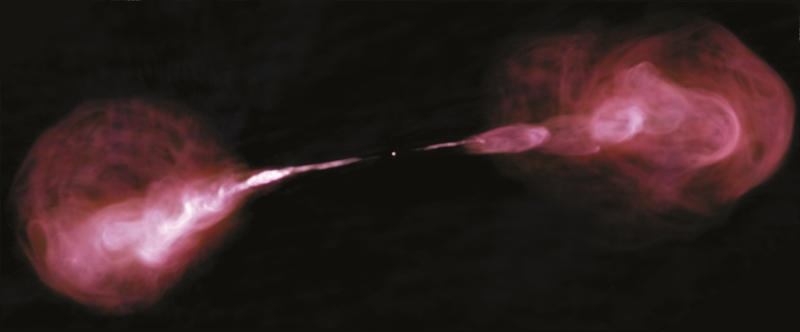
\includegraphics[width=0.8\textwidth]{images/herculesA.jpg}
  \caption{Hercules A, a radio galaxy. We see jets emitted from the supermassive
    black hole near the centre of the image. The galaxy itself is not visible in
    radio wavelengths. \emph{Image: B. Saxton, W. Cotton and R. Perley
    (NRAO/AUI/NSF)}}
  \label{fig:radio-galaxy}
\end{figure}

Objects detected by EMU will need to be cross-identified with their counterparts
in surveys at other wavelengths. Unfortunately, radio objects can be arbitrarily
complex --- many radio objects are jets from supermassive black holes at the
centre of galaxies, and these jets warp as they interact with their environment.
An example of such an object is shown in Figure \ref{fig:radio-galaxy}. An
estimated 10\% of EMU radio objects will be too complicated for current
automated cross-identification algorithms \citep{banfield15, norris11}.

\citet{banfield15} created Radio Galaxy Zoo to attempt to address this
problem. Radio Galaxy Zoo is a citizen science project based on the highly
successful Galaxy Zoo \citep{lintott08, lintott11}. The Zooniverse
platform\footnote{\url{http://zooniverse.org/}} created by Galaxy Zoo provides a
way for non-experts to help researchers label data across a wide range of
scientific fields, and has resulted in well over 110 publications. In the case
of Radio Galaxy Zoo, volunteers are invited to cross-identify radio objects
imaged by the NRAO Very Large Array and the Australia Telescope with their
infrared counterparts imaged by the Wide-area Infrared Survey Explorer (WISE)
and Spitzer telescopes. The cross-identification interface is available online
for anyone to use\footnote{\url{http://radio.galaxyzoo.org/}}. To date, with the
help of thousands of volunteers, Radio Galaxy Zoo has managed to cross-identify
over 100 000 radio galaxies. This still does not compare in scale to EMU, but
the hope is that these cross-identification labels can be used to train
next-generation machine learning algorithms.

This thesis presents a na\"ive, supervised learning approach to the problem of
active galactic nuclei cross-identification, using label data sourced from the
Radio Galaxy Zoo.

\section{Contributions}
\label{sec:contributions}

  \begin{itemize}
    \item ML on RGZ
    \item Non-physical model for cross identification
    \item Deep learning features for radio
    \item Effect of features. \url{https://see.stanford.edu/materials/aimlcs229/ml-advice.pdf}
    \item Framing cross identification as object localisation then binary classification
    \item Implementation of Raykar and Yan
    \item Compare Raykar, Yan, MV (wins)
    \item Compare Logistic Regression with Random Forest
    \item Benefit active learning
  \end{itemize}

\section{Outline}
\label{sec:outline}
  
  Chapter \ref{cha:astro} introduces astronomical concepts such as radio active
  galactic nuclei. These concepts are important to understand both the purpose
  of this thesis, and to understand the problem we are trying to solve. We also
  introduce four astronomical surveys --- EMU, ATLAS, WISE, and SWIRE --- that
  produced the data we used in our experiments.

  Chapter \ref{cha:ml} introduces machine learning concepts such as
  classification and image feature extraction. These concepts are the building
  blocks for a machine-learned algorithm for automated radio
  cross-identification. We also perform some experiments to test how selected
  crowd learning algorithms behave in different contexts.

  Chapter \ref{cha:cross-identification} brings together Chapters 2 and 3 to
  develop a machine learning approach to the radio cross-identification task. We
  formalise the problem and highlight the problems that must be solved for
  development, trial different methods of approaching the task, and present
  results on task performance using our classifier.

  Chapter \ref{cha:active-learning} discusses active learning, and its
  application to crowdsourced projects like the Radio Galaxy Zoo. We perform
  some simple experiments and suggest future pathways for research in this area.

  Appendix \ref{cha:crowdastro} describes crowdastro, a Python package developed
  as part of this project. This package was used to perform all experiments
  described in this thesis. It also provides a command-line interface for
  training and executing the automated cross-identification task.

\section{Data Products and Packages Used in this Thesis}
\label{sec:data-products}
  
  The work presented in this thesis would not have been possible without the
  various data products used for experiments and development.

  This thesis makes use of data products from the Wide-field Infrared Survey
  Explorer (WISE), the Spitzer Space Telescope, and the Australia Telescope
  Compact Array. WISE is a joint project of the University of California, Los
  Angeles, and the Jet Propulsion Laboratory/California Institute of Technology,
  funded by the National Aeronautics and Space Administration. The Spitzer Space
  Telescope is operated by the Jet Propulsion Laboratory, California Institute
  of Technology, under contract with NASA. SWIRE was supported by NASA through
  the Spitzer Legacy Program under contract 1407 with the Jet Propulsion
  Laboratory. The Australia Telescope Compact Array is part of the Australia
  Telescope, which is funded by the Commonwealth of Australia for operation as a
  National Facility managed by CSIRO.

  This thesis also makes use of the Breast Cancer Wisconsin dataset. The dataset
  was obtained from the University of Wisconsin Hospitals, Madison from Dr.
  William H. Wolberg, and was accessed from the UCI Machine Learning Repository
  \footnote{https://archive.ics.uci.edu/ml/}.

  This thesis made use of astropy \citep{astropy}, a community-developed core
  Python package for astronomy, and scikit-learn \citep{scikit-learn}, an open
  source package machine learning package.

  Finally, this thesis had been made possible by the participation of more then
  10~000 volunteers in the Radio Galaxy Zoo project. Their contributions are
  individually acknowledged at http://rgzauthors.galaxyzoo.org.

%!TEX root=thesis.tex
\chapter{Galaxies and Active Galactic Nuclei}
\label{cha:astro}

    Modern astronomy relies on observations of deep space. Telescopes image the
    sky in different wavelengths, with different wavelengths carrying different
    physical meanings. Infrared surveys detect star formation and dust in
    distant galaxies, and radio surveys detect massive objects called active
    galactic nuclei. In this section, we describe what we see when we look at
    the sky in these wavelengths, as well as introducing specific radio and
    infrared surveys relevant to this thesis. We also discuss the motivation
    behind cross-identifying active galactic nuclei with their host galaxies, as
    well as the inherent difficulty in doing so, and hence provide the
    motivation behind this thesis.

    \section{Radio Active Galactic Nuclei}
    \label{sec:agns}

        \begin{figure}[!ht]
            \centering
            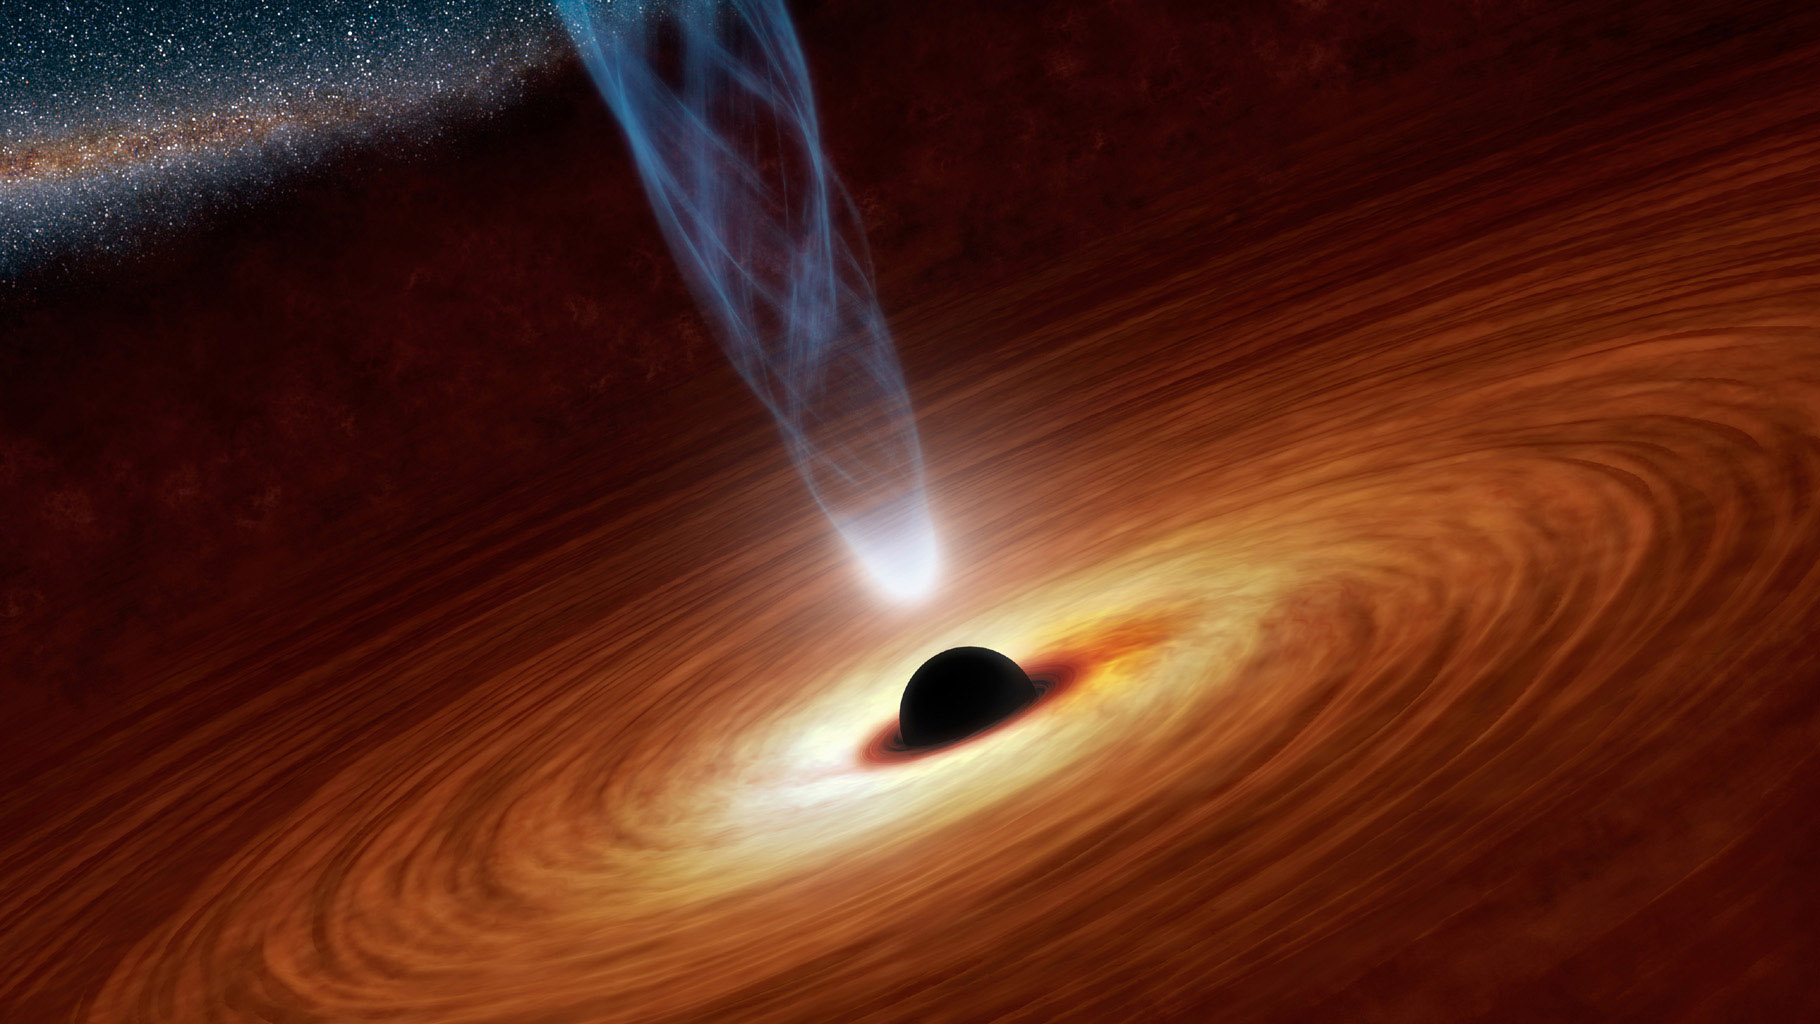
\includegraphics[width=0.8\textwidth]
                {images/accretion_disk_artist_impression.jpg}
            \caption{An artist's impression of the accretion disk of an active
                galactic nucleus. \emph{Image: NASA/JPL-Caltech}}
            \label{fig:accretion-disk}
        \end{figure}

        Many galaxies contain a supermassive black hole in their centre. These
        black holes accrete matter from the surrounding galaxy in an
        \emph{accretion disk} (Figure \ref{fig:accretion-disk}). The accretion
        process emits huge amounts of light through different physical
        processes. These light-emitting black holes are called active galactic
        nuclei (AGNs). AGNs can be extremely bright, emitting up to $10^{39}$ J
        of energy every second --- nearly a thousand times more energy than our
        entire galaxy emits \citep{begelman84}. AGNs are found throughout the
        universe: The closest known AGN is Centaurus A (shown in Figure
        \ref{fig:centaurus-a}), with $z \approx 0.0018$, and AGNs have been
        detected up to redshifts of $z \approx 7$ \citeme.

        \begin{figure}[!ht]
            \centering
            \includegraphics[width=0.5\textwidth]
                {images/ESO_Centaurus_A_LABOCA.jpg}
            \caption{Centaurus A, a relatively close radio active galactic
                nucleus. \emph{Image: ESO/WFI (Optical); MPIfR/ESO/APEX/A.Weiss
                et al. (Submillimetre); NASA/CXC/CfA/R.Kraft et al. (X-ray)}}
            \label{fig:centaurus-a}
        \end{figure}

        AGNs produce \emph{jets} from their accretion disk. Jets are long, thin
        streams of matter such as the one shown in Figure \ref{fig:m87}. These
        jets can be very long, with ``giant'' AGNs emitting jets nearly 1 Mpc in
        length \citep{saripalli05}. The process through which jets are emitted
        is currently unknown \citeme.

        \begin{figure}[!ht]
            \centering
            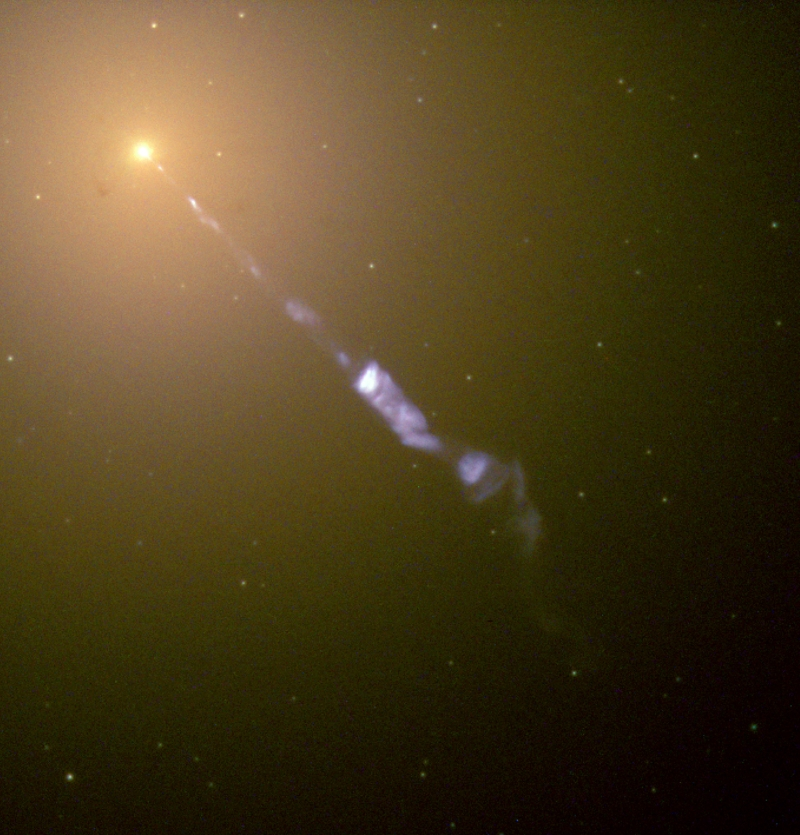
\includegraphics[width=0.5\textwidth]{images/M87_jet.jpg}
            \caption{M87, a giant elliptical galaxy with a jet. \emph{Image:
                NASA and The Hubble Heritage Team (STScI/AURA)}}
            \label{fig:m87}
        \end{figure}

        Electrons in jets can produce \emph{synchrotron radiation}, a form of
        radiation emitted by charged particles as they accelerate at
        relativistic speeds in a magnetic field \citeme. This
        radiation is emitted in radio wavelengths, and so AGNs emitting this
        kind of radiation are called \emph{radio AGNs}. As radio AGNs are the
        focus of this thesis, from this point on ``AGN'' will refer only to
        radio AGNs.

        To fully understand these objects, astronomers need data from more than
        just radio surveys. Combining observations of objects in multiple
        wavelengths is thus a common problem in astronomy, and is called
        \emph{cross-identification} \citep{fan15}. For point sources of light,
        this can be straightforward --- the coordinates of each source on the
        sky are well-known and can often be immediately matched throughout
        surveys --- but as we can only observe AGNs by observing their jets,
        AGNs are effectively not point sources. We discuss this in detail in
        Section \ref{sec:radio-cross-identification}.

    \section{Astronomical Observations}
    \label{sec:astronomical-observations}

        When observing the sky, we can think about the sky as a spherical
        surface surrounding the earth. All objects we see with telescopes are
        flat on the sky, and we only have limited tools to determine their
        distances and scales. In this section, we describe the coordinate
        systems and units used to describe these objects.

        \subsection{Astronomical Coordinates}
        \label{sec:coordinates}

            Astronomy uses a coordinate system called the \emph{equatorial
            coordinate system} to describe the positions of objects on the sky.
            Each position on the sky is described by two numbers: the
            \emph{right ascension} (RA) and the \emph{declination} (dec).

            \begin{figure}[!ht]
                \centering
                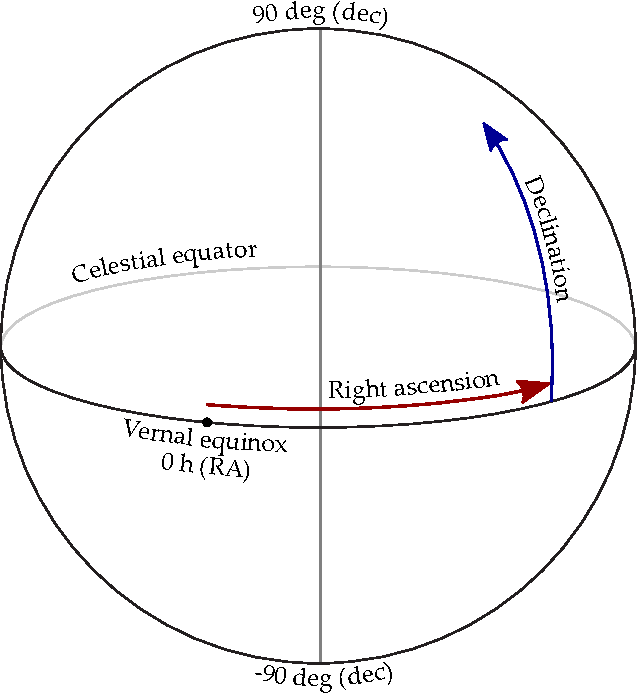
\includegraphics[width=0.5\textwidth]{images/ra-dec}
                \caption{The equatorial coordinate system.}
                \label{fig:equatorial-coordinates}
            \end{figure}

            The right ascension of an object is the angle eastward from the
            vernal equinox to the object along the celestial equator. It is
            measured in hours (h), minutes (min), and seconds (s). There are 60
            seconds in 1 minute, 60 minutes in 1 hour, and 1 hour is equal to 15
            degrees. Right ascension ranges between 0h and 24h, where both 0h
            and 24h are located at the vernal equinox. The declination of an
            object is the angle northward from the celestial equator to the
            object. It is measured in degrees (${}^\circ$), arcminutes ($'$),
            and arcseconds ($"$). Declination ranges between $-90^\circ$ and
            $90^\circ$, where $-90^\circ$ is the declination of the south
            celestial pole and $90^\circ$ is the declination of the north
            celestial pole. The right ascension and declination are shown in
            Figure \ref{fig:equatorial-coordinates}. It is important to note
            that while right ascension and declination are both measured in
            minutes and seconds, these are \emph{different} minutes and seconds.
            1 minute (right ascension) is equal to 15 arcminutes (declination).

            Objects are usually given a International Astronomical Union (IAU)
            name based on their coordinates. This name includes the catalogue
            that identified the object, the right ascension, and the
            declination. For example, ATLAS3 J002925.7-440256C is from the third
            release of the ATLAS catalogue, and is located at 00h 29m 25.7s
            $-44^\circ$ $02'$ $56"$.

        \subsection{Wavelength and Frequency}
        \label{sec:wavelength}

            \emph{Wavelength} is a property of radiation corresponding to its
            colour. Wavelength is measured in metres (m) and is usually denoted $\lambda$. Ranges of wavelengths are given common names such as
            infrared, optical, and radio.

            When objects emit radiation, the wavelength of the emitted radiation
            depends on the process by which it was emitted. For example, thermal
            radiation is emitted by all objects based entirely on the
            temperature of the object, with hotter objects emitting light with
            shorter wavelengths. Another example is synchrotron radiation
            (Section \ref{sec:agns}), which is emitted in radio wavelengths.

            Since telescopes generally only detect brightnesses of objects in
            the sky, and different wavelengths of radiation require different
            mechanisms to detect, telescopes are designed to measure radiation
            only at specific ranges of wavelengths. Separate measurements of
            wavelength are later combined for analysis.

            \emph{Frequency} is another common property of radiation. It is
            measured in hertz (Hz) and usually denoted $\nu$. Wavelength and
            frequency are interchangeable using the formula
            \[
                c = \lambda \nu
            \]
            where $c$ is the speed of light.

        \subsection{Flux and Magnitude}

            The \emph{flux density} $f$ of an object is its energy output per
            unit time per unit area, and is measured in $\text{W m}^{-2}$. The
            flux density is given by
            \[
                f = \frac{1}{A}\frac{\text{d}E}{\text{d}t}
            \]
            We cannot usually measure the flux over all frequencies, so usually
            flux is observed over a specific frequency range $\Delta \nu$. The
            \emph{spectral flux density} is then the limit of this as the
            frequency range approaches zero, i.e.
            \[
                f_\nu = \frac{1}{A}\frac{\text{d}^2E}{\text{d}\nu\text{d}t}
            \]
            where $E$ is the energy received from the object, $A$ is the area of
            the object on the sky, and $\nu$ is the frequency. The spectral flux
            density is measured in janskys (Jy), an astronomical unit equal to
            $10^{-26} \text{ W m}^{-2} \text{ Hz}^{-1}$ \citep{francis08}.

            The \emph{apparent magitude} $m$ of an object is a logarithmic
            measure of its apparent brightness seen from Earth, relative to the
            star Vega \citep{francis08}. The difference between the magnitudes
            of two objects represents the ratio of their flux densities
            \begin{equation}
                \label{eq:magnitude-difference}
                m_2 - m_1 = -2.5 \log_{10} \left(\frac{f_2}{f_1}\right)
            \end{equation}
            and so the apparent magnitude is given by
            \begin{equation}
                \label{eq:apparent-magnitude}
                m = -2.5 \log_{10} \left(\frac{f}{f_{\text{Vega}}}\right)
            \end{equation}
            where $f$ is the flux density of the object and $f_{\text{Vega}}$ is
            the flux density of Vega, measured at the same frequency.

    \section{Radio Surveys}
    \label{sec:radio-surveys}

        A \emph{survey} is an image of the sky made with repeated observations
        in specific wavelengths, aiming to comprehensively cover some large area
        of the sky. In this section we look at EMU and ATLAS, two surveys in
        radio wavelengths that are relevant to this thesis.

        \begin{figure}[!ht]
            \centering
            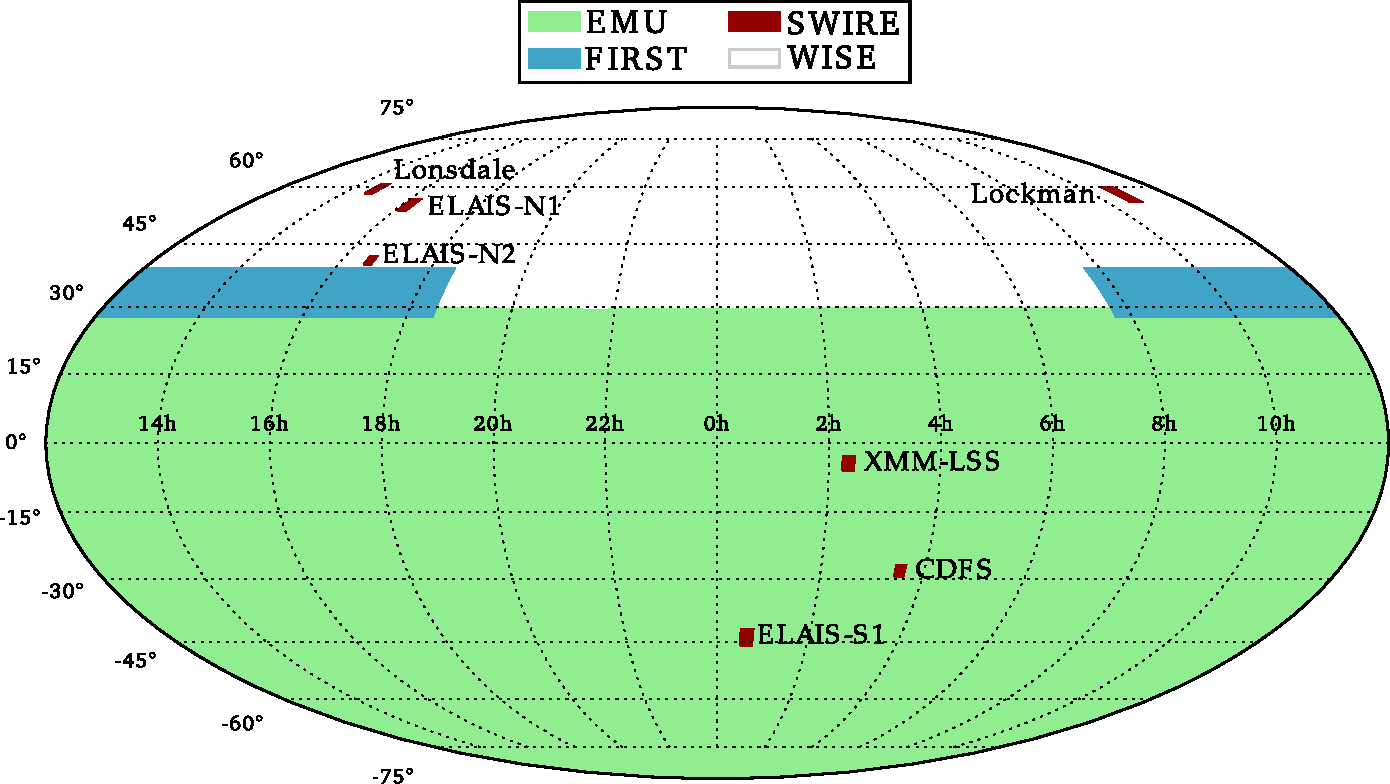
\includegraphics[width=0.8\textwidth]{images/skymap.pdf}
            \caption{A map of the sky, showing the FIRST and EMU radio surveys,
                and the WISE and SWIRE infrared surveys. The ATLAS radio survey
                covers both the CDFS and ELAIS-S1 fields.}
        \end{figure}

        \subsection{EMU: Evolutionary Map of the Universe}
        \label{sec:emu}

            The largest existing radio survey is currently the NRAO VLA Sky
            Survey (NVSS) \citep{condon98}, which covered the entire northern
            sky as far south as $-40^\circ$. However, NVSS is very shallow, only
            detecting objects brighter than $2.5$ mJy, and only resolving
            objects to $45''$. The deepest existing radio survey is of the SWIRE
            fields \citep{owen08}, which only covered around $0.1$ deg$^2$ of
            the sky, but to a depth of $0.015$ mJy with an angular resolution of
            $1.6''$. The Evolutionary Map of the Universe (EMU) is an upcoming
            deep radio survey that aims to provide both deep and wide coverage
            of the radio sky \citep{norris11}. EMU will be sensitive to objects
            to around $0.015$ mJy with an angular resolution of around $10''$,
            and cover the entire southern sky as far north as $30^\circ$. The
            survey is expected to find huge numbers of radio objects --- while
            ATLAS (Section \ref{sec:atlas}) has detected around 4000 radio
            objects, EMU is expected to find \emph{70 million} \citep{banfield15}. Such large
            numbers of radio objects make analysis of the data considerably more
            difficult than analysis of existing surveys has been. Analysis of
            EMU is far too large to be done by hand, and as such will require
            algorithms to process the data. With such large numbers of new
            objects, it is likely that many objects will not fit existing
            models, meaning that model-based approaches to data processing may
            be ineffective. It is this problem that motivates the development of
            new, machine-learned algorithms for processing astronomical data at
            these large scales. While the EMU survey data is not yet released,
            development of such algorithms can begin by looking at other
            datasets with similar sensitivity and resolution, such as ATLAS
            (Section \ref{sec:atlas}).

            EMU aims to fulfil a number of scientific goals, including:
            \begin{itemize}
                \setlength\itemsep{0 pt}
                \item investigating the evolution of galaxies and supermassive
                    black holes,
                \item exploring the large-scale structure and cosmology of the
                    universe,
                \item developing a catalogue of radio objects in the southern
                    sky,
                \item looking for never-before-seen astronomical objects, and
                \item testing strategies for dealing with data from the upcoming
                    Square Kilometre Array (SKA) telescope.
            \end{itemize}

        \subsection{ATLAS: The Australia Telescope Large Area Survey}
        \label{sec:atlas}

            \begin{figure}[!ht]
              \centering
              \includegraphics[width=0.8\linewidth,]{images/CDFS_bitmap}
              \caption{ATLAS observations of CDFS. Reproduced from \citet{franzen15}.}.
              \label{fig:cdfs}
            \end{figure}

            The Australia Telescope Large Area Survey (ATLAS) is a deep survey
            of two small areas of the sky in radio wavelengths, which aims to
            help understand the evolution of early galaxies \citep{norris06}.
            The Australia Telescope Compact Array was used to image the Chandra
            Deep Field South (CDFS) and the European Large Area ISO Survey -
            South 1 (ELAIS-S1) fields. These fields are areas of the sky with
            few nearby objects, meaning that observations in these fields are of
            very old, distant objects. These fields were chosen because they are
            the two fields imaged in the Spitzer Wide-area Infrared
            Extragalactic Survey (SWIRE, Section \ref{sec:swire}) visible from
            the southern hemisphere. SWIRE produced high-resolution infrared
            images of its fields, allowing all objects detected in the ATLAS
            radio images to be cross-identified with their infrared
            counterparts.

            ATLAS is considered a pilot survey for EMU. EMU and ATLAS image the
            same wavelengths with similar resolution and sensitivity, so tools
            and methods developed to process and interpret ATLAS data are
            expected to work well on the data produced by EMU.

            ATLAS provides both a catalogue of detected radio objects and a
            radio image of the CDFS and ELAIS-S1 fields. The CDFS image covers a
            total area of 3.7 deg$^2$ and the ELAIS-S1 image covers a total area
            of 2.7 deg$^2$. The CDFS image is shown in Figure \ref{fig:cdfs}.
            The catalogue is a list of all objects detected in the images with a
            peak or integrated flux more than 5 times the background noise
            levels. Each object has an associated survey identifier, an IAU
            name, a position on the sky of the peak flux, a peak flux density,
            an integrated flux density, an angular size, whether the object is
            extended or compact, and a spectral index, as well as uncertainties
            associated with each measurement \citep{franzen15}.

    \section{Infrared Surveys}
    \label{sec:infrared-surveys}

        \subsection{WISE: Wide-field Infrared Survey Explorer}
        \label{sec:wise}

            \begin{figure}[!ht]
                \centering
                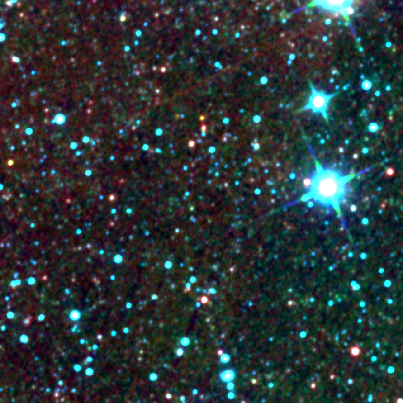
\includegraphics[width=0.5\textwidth]
                    {images/WISE_3h30m05.24s-28d34m46.3s.png}
                \caption{Patch of the WISE multi-wavelength composite image
                    centred on 3h30m05.24s -28d34m46.3s.}
                \label{fig:wise}
            \end{figure}

            The Wide-field Infrared Survey Explorer (WISE) is an orbital
            infrared telescope. In 2009--2010 it was used to survey the entire
            sky in four wavelengths, 3.4 $\mu$m, 4.6 $\mu$m, 12 $\mu$m, and 22
            $\mu$m. These wavelengths are referred to as WISE bands $w1$, $w2$,
            $w3$, and $w4$, respectively. WISE images have resolutions of
            $6''$--$12''$, with sensitivity between $0.08$ and $6$ mJy,
            corresponding to the detection of sources between $16.5$ and $7.9$
            magnitude \citep{wright10}.

            The main goal of the WISE survey is to provide a map of the whole
            sky in infrared wavelengths for many different reasons: infrared
            measurements may be used to detect and classify distant galaxies,
            measurements can be cross-identified to complement other surveys,
            and so on. There are many other scientific goals of WISE; these are
            described in detail by \citet{wright10}.

        \subsection{SWIRE: Spitzer Wide-Area Infrared Extragalactic Survey}
        \label{sec:swire}

            \begin{figure}[!ht]
                \centering
                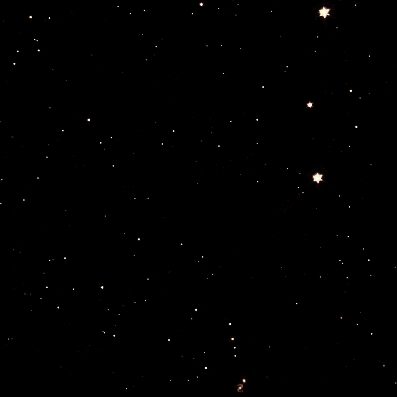
\includegraphics[width=0.5\textwidth]{images/swire_small.jpg}
                \caption{Patch of the SWIRE multi-wavelength composite image
                    centred on 3h30m05.24s -28d34m46.3s. This is the same region
                    of the sky as the WISE image in Figure \ref{fig:wise}.}
            \end{figure}

            The Spitzer Wide-Area Infrared Extragalactic Survey (SWIRE) is an
            infrared survey of seven fields of the sky
            \citep{lonsdale03}. These fields --- ELAIS-S1, ELAIS-N1, ELAIS-N2,
            Lockman, CDFS, and Lonsdale --- are called the \emph{SWIRE fields},
            totalling 63.2 $\deg^2$ in area. ELAIS-S1 and CDFS are in the
            southern sky; all other fields are in the northern sky. SWIRE is a
            multi-wavelength survey, observing at four wavelengths: 3.6 $\mu$m,
            4.5 $\mu$m, 5.8 $\mu$m, and 8.0 $\mu$m.

            While SWIRE covers far less area of the sky than WISE, it does so at
            considerably higher resolution and sensitivity: \todo{Find
            resolution of SWIRE} and $7.3 - 32.5$ $\mu$Jy, respectively.

            SWIRE aimed to investigate the evolution of galaxies and AGNs and
            the relationship between galaxies and AGNs \citep{surace05}.

    \section{Radio Cross-identification}
    \label{sec:radio-cross-identification}

        \subsection{Motivation}
        \label{sec:cross-identification-motivation}

        The main goal of cross-identifying AGNs is to better understand the
        relationship between AGNs and star-forming activity in their host
        galaxies \citep{norris06}.

        While we cannot observe the black holes of AGNs directly, we can observe
        the radio emissions from their jets. These could then be matched to the
        galaxies hosting the black holes, allowing us to learn more about the
        galaxy, the black hole, and the surrounding environment. These host
        galaxies are not visible in radio wavelengths,

        \todo{Rewrite + finish}

        \subsection{Norris et al. Catalogue}
        \label{sec:norris}

            \begin{itemize}
                \item Norris provided a catalogue of cross-identifications
                \item The catalogue is ``expert'' data, so sorted through by actual astronomers
                \item The catalogue contains the names and locations of each component and matches them to the corresponding SWIRE objects
                \item The catalogue also contains the flux associated with the SWIRE object
                \item Estimated $9.02\%$ false cross-identifications
            \end{itemize}

        \subsection{Fan et al. Catalogue}
        \label{sec:fan}

            \begin{itemize}
                \item Bayesian hypothesis testing to fit models to the ATLAS catalogue
                \item Doesn't detect IR sources not in catalogue
                \item Matches within 2'
                \item Matched 564 radio objects identically to Norris, missed 31 Norris identified, and identified an additional 62
            \end{itemize}

    \section{Radio Galaxy Zoo}
    \label{sec:radio-galaxy-zoo}

        \begin{itemize}
            % \item The Norris catalogue is manual expert classifications, which scales terribly (especially for EMU)
            % \item The Fan catalogue is model-based, so might miss things that are unusual
            % \item Radio Galaxy Zoo is an attempt to generate a catalogue of cross-identifications for the ATLAS and FIRST surveys using crowdsourcing
            % \item This is an example of citizen science, see also Lintott et al. Galaxy Zoo
            % \item Aims to have non-experts classify radio objects \cite{norris16}
            % \item 20 classifications for complex objects, 5 for compact \cite{banfield15}
            \item Launched in December 2013
            \item Resulted in x cross-identifications of FIRST and ATLAS
            \item Brief description of how it works
            \item Citizen scientists also found one of the largest known WATs \cite{banfield16}
            \item The plan is to use RGZ as a training set for next-generation cross-identification and classification algorithms
        \end{itemize}

    The \citeauthor{norris06} catalogue is highly accurate, but manual expert
    cross-identification of radio surveys is impractical for large surveys. The
    CDFS field examined by \citeauthor{norris06} only contains around 2400 radio
    objects, which is small even compared to existing surveys --- FIRST
    \citep{becker95} found 946 000 radio sources, and EMU is expected to find 70
    million. Automated algorithms such as \citeauthor{fan15} scale better, but
    most such algorithms are still in their infancy \citeauthor{norris16} and
    many are model-based, potentially missing many sources that do not fit the
    models. The Radio Galaxy Zoo project \citep{banfield15} provides a different
    approach: Allow many non-expert volunteers to manually cross-identify radio
    sources with their infrared host galaxies.

    Radio Galaxy Zoo is a website where volunteers are presented with a radio
    image from ATLAS or FIRST and a corresponding infrared image from SWIRE or
    WISE, and are tasked with matching the radio source with its host galaxy, as
    well as identifying which radio objects are associated with the same host
    galaxy (e.g., two radio objects may represent two jets of one AGN). While
    both the cross-identification task and the radio object association task are
    astronomically interesting, we focus only on the cross-identification task
    for this thesis. An example of the workflow presented to volunteers is shown
    in Figure \ref{fig:rgz-interface}.

    Since its launch in December 2013, the Radio Galaxy Zoo project has labelled over 100 000 radio objects. One particularly notable result is the discovery of one of the largest known wide-angled tail AGNs by two citizen scientists, which would be impossible to detect in current automated algorithms \citep{banfield16}.

    \begin{figure}[!ht]
        \centering
        \begin{subfigure}[t]{0.3\textwidth}
            \centering
            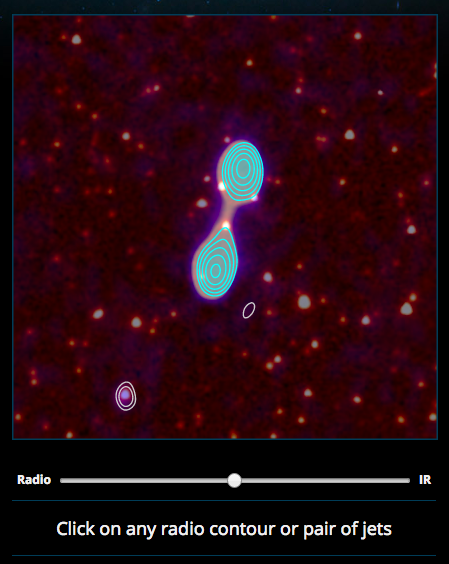
\includegraphics[height=2in]{images/rgz_radio.png}
            % These empty captions give us something to reference later.
            \caption{}
            \label{fig:rgz-interface-a}
        \end{subfigure}%
        ~
        \begin{subfigure}[t]{0.3\textwidth}
            \centering
            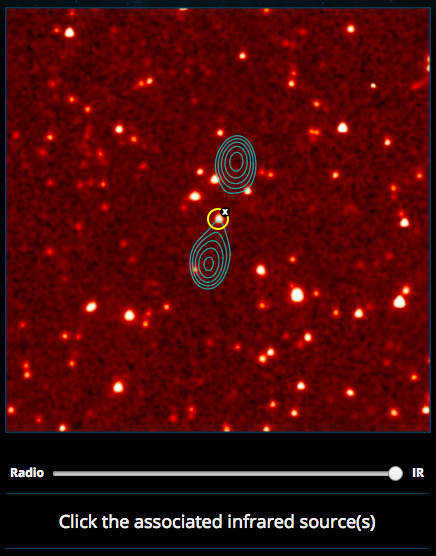
\includegraphics[height=2in]{images/rgz_ir.png}
            \caption{}
            \label{fig:rgz-interface-b}
        \end{subfigure}%
        ~
        \begin{subfigure}[t]{0.3\textwidth}
            \centering
            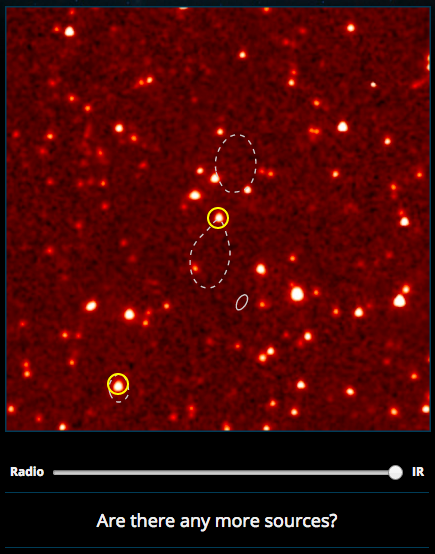
\includegraphics[height=2in]{images/rgz_done.png}
            \caption{}
            \label{fig:rgz-interface-c}
        \end{subfigure}
        \caption{Radio Galaxy Zoo volunteer workflow.\\\ref{fig:rgz-interface-a}
          Volunteers are first asked to identify associated radio objects.
          \\\ref{fig:rgz-interface-b} Volunteers then cross-identify the radio
          objects with the corresponding host galaxy.\\\ref{fig:rgz-interface-c}
          This is repeated for all radio objects in the image.}
        \label{fig:rgz-interface}
    \end{figure}

    The Radio Galaxy Zoo dataset contains around 177 000 images from FIRST, and
    2400 images of the CDFS field from ATLAS. The ATLAS images of the ELAIS-S1
    field are not included, and may be used as a testing set for cross-%
    identification algorithms trained on the Radio Galaxy Zoo in the future.
    Each image is a 2 arcminute-wide square.

    To help reduce noise in the labels, each compact radio object is shown to 5
    volunteers, and each complex radio object is shown to 20 volunteers.

    The labels are stored in a MongoDB database as a collection of associated
    radio objects and the corresponding pixel locations that volunteers clicked
    on, as well as the right ascension and declination of the radio object. The
    radio and infrared image patches associated with each radio object are also
    included alongside the database.

    In this thesis, we will train machine learning algorithms to perform the
    cross-identification task trained on ATLAS-CDFS labels from the Radio Galaxy
    Zoo.

%     Radio Galaxy Zoo volunteers are first asked to select combinations of
%     radio objects that correspond to one radio source, and are then asked to
%     select the location of the corresponding host galaxy \citep{banfield15}.
%     Each radio subject is labelled by multiple volunteers. These labels are
%     then collated as follows. First, the most common combination of radio
%     objects is selected, and all labels that have a different combination are
%     discarded. This radio combination is called the consensus radio
%     combination. Then, the density of host location labels is estimated using
%     Gaussian kernel density estimation (KDE), and the highest density location
%     is selected. This is called the consensus host location. The consensus
%     host location is then matched to the nearest infrared object.

%     An alternative way to find the consensus host location is by using a
%     clustering algorithm such as $k$-means. Host locations are clustered and
%     the cluster containing the most locations is taken to represent the
%     consensus; the consensus location is then the mean of the cluster. This is
%     faster and more robust than using KDE, but requires $k$ to be known. $k$
%     can be estimated using an algorithm such as PG-means \citep{hamerly07} or
%     by choosing $k$ to minimise some information criterion
%     \todo{cite:sklearn}. The consensus labels for the data associated with
%     this thesis were found in this way, fitting a Gaussian mixture model to
%     the host locations with the number of Gaussians chosen to minimise the
%     Bayesian information criterion.

%     Repeated volunteer labelling helps to reduce noise in the labels. This is
%     necessary as the volunteers are not experts, and may incorrectly label the
%     subject. The hope is that the majority of volunteers will correctly label
%     subjects, which seems to be the case for radio subjects where more than
%     75\% of volunteers agree \citep{banfield15}. The number of times a radio
%     subject is shown to different volunteers is called the redundancy. The
%     redundancy is 5 if the subject is a compact source, and 20 for all other
%     sources. These numbers were chosen based on the redundancy levels of the
%     original Galaxy Zoo project [Banfield, personal communication] \todo{Is
%     this how to cite personal communication? Alternatively, is this written
%     down somewhere?}. Since labels with radio combinations that disagree with
%     the consensus are discarded, the redundancy is usually lower in practice
%     when finding the host location. This can lead to very low redundancy input
%     to KDE, causing KDE to fail. This failure can usually be caught, but the
%     existing solution in this case is to take the mean of all host locations.
%     This is not the consensus host location in general. Another effect is that
%     since more complex sources have higher levels of disagreement in the radio
%     combination stage, more complex sources have more discarded volunteer
%     labels, and thus lower redundancy --- so more complex sources have more
%     noise in their labels.

%!tex root=thesis.tex
\chapter{Machine Learning on Crowds}
\label{cha:ml}

In this chapter we will discuss machine learning. While we introduce a number of
concepts that will help us develop our cross-identification method, we will not
yet apply these concepts to astronomical data, instead deferring this to Chapter
\ref{cha:cross-identification}.

In Section \ref{sec:classification}, we introduce the problem of classification,
and discuss some common methods of approach. We will later base our
cross-identification methods on these.

In Section \ref{sec:image-feature-extraction}, we look at automated feature
extraction from images. Convolutional neural networks will be introduced as
feature extractors, which we will eventually apply to radio data from ATLAS.

In Section \ref{sec:crowdsourcing}, we discuss the benefits and problems of
crowdsourcing for obtaining labels for machine learning. Finally, we will then
look at different ways to handle the problems in Section \ref{sec:crowd-labels}.

\section{Classification}
\label{sec:classification}

    A common machine learning task is \emph{classification}. Given a set
    $\mathcal X$ of \emph{instances} and a set $\mathcal Y$ of \emph{labels},
    the classification task is to assign a label $y \in \mathcal Y$ to each
    instance $x \in \mathcal X$. Effectively, we want to find a map $y :
    \mathcal X \to \mathcal Y$.

    The ``true'' label of an instance is called the \emph{groundtruth}, and is
    denoted $z$. Classification thus amounts to modelling the conditional
    distribution $p(z \mid x)$. An example of classification is labelling images
    of digits, where $\mathcal X$ is a set of images and $\mathcal Y = \{0,
    \dots, 9\}$ \citep{lecun98}. A less obvious example is that of diagnosing
    breast cancer in patients, where $\mathcal X$ is a set of sets of medical
    observations and $\mathcal Y$ is the set $\{\text{malignant},
    \text{benign}\}$ \citep{wolberg90}.

    Modelling $p(z \mid x)$ requires some set of \emph{training data} $\mathcal
    D \subset \mathcal X \times \mathcal Y$. The training data are either used
    to find parameters for a model or to estimate the model directly. Both
    processes are called \emph{training} the model. The cardinality of the
    training data is denoted $N = |\mathcal D|$.

    \emph{Binary classification} is classification where each instance must be
    assigned one of two labels, i.e. $\mathcal Y \sim \{0, 1\}$. Instances with
    a true label of $0$ are called \emph{negative instances}, and instances with
    a true label of $1$ are called \emph{positive instances}. For this thesis,
    we will focus entirely on binary classification and set $\mathcal Y = \{0,
    1\}$.

    Instances are usually represented by a vector of \emph{features}, denoted
    $\vec x$. Choosing features is an important and non-trivial part of
    modelling a classification task, and can strongly affect the ability of a
    model to classify instances. The dimensionality of the feature space is
    denoted $D$ and we assume that $\mathcal X \subseteq \mathbb{R}^D$.

    We will now look at how to evaluate a classification model, and introduce
    three common ways of modelling binary classification: logistic regression,
    neural networks, and random forests.

    \subsection{Evaluating a Classification Model}
    \label{sec:evaluating-classification-model}

        Given a classification model $y(\vec x)$ that aims to approximate $p(z
        \mid \vec x)$, we want to know how well this model represents the
        groundtruth. In this thesis we make use of two evaluation metrics:
        cross-entropy error, and balanced accuracy.

        The \emph{cross-entropy error} \citep{bishop06} is a common method for
        evaluating a binary classification model. The cross-entropy error is
        given by
        \[
            L(\mathcal D) = -\frac{1}{N} \sum_{\vec x, z \in \mathcal D} \left(
                z \log y(\vec x) + (1 - z) \log (1 - y(\vec x))
            \right).
        \]
        Higher error indicates a ``worse'' model.

        The \emph{balanced accuracy} is another common method of evaluating
        classification models. It is the average of the accuracy of classifying
        positive instances and the accuracy of classifying negative instances,
        i.e.
        \[
            a = \frac{1}{2} \left(\frac{p_{\text{true}}}{p} + \frac{n_{\text{true}}}{n}\right),
        \]
        where $p$ is the number of instances with $z = 1$, $n$ is the number of
        instances with $z = 0$, $p_{\text{true}}$ is the number of correctly
        classified instances with $z = 1$, and $n_{\text{true}}$ is the number
        of correctly classified instances with $z = 0$.

        Unless otherwise specified, we use the cross-entropy error for training
        our models, and report the balanced accuracy.

    \subsection{Logistic Regression}
    \label{sec:logistic-regression}

        Logistic regression is a simple linear model of binary classification
        \citep{bishop06}. The conditional distribution $p(z \mid \vec x)$ is
        modelled as
        \begin{equation}
            \label{eq:logistic-regression}
            y(\vec x) = p(z = 1 \mid \vec x) = \sigma(\vec w^T \vec x + b),
        \end{equation}
        where $\vec w$ and $b$ are parameters to the model and $\sigma$ is the
        logistic sigmoid function
        \[
            \sigma(t) = \frac{1}{1 + \exp(-t)}.
        \]
        The elements of $\vec w$ are called the \emph{weights}, and control the
        effect of each feature on the output label probability. $b$ is the
        \emph{bias}, a constant added to all weighted sums of features
        independent of the features themselves. $b$ can be incorporated into
        $\vec w$ by adding an extra feature to $\vec x$ that is always $1$ and
        increasing the dimension of $\vec w$ by 1. We will adopt this convention
        whenever $b$ is not explicitly included.

        Logistic regression is one of the simplest models we can make, and is
        the classification analogue of linear regression. We can think of it as
        a linear function with a ``soft'' threshold, with all output values
        above the threshold approaching $1$ and all other outputs approaching
        $0$. The logistic sigmoid function causes this threshold effect. While
        we could instead use a step function, a differentiable function like the
        logistic sigmoid function means that logistic regression will be
        differentiable.

        Since logistic regression is differentiable, \emph{gradient descent} can
        be used to find optimum values of $\vec w$. $\vec w$ is modified by the
        update equation
        \[
            \vec w_{t+1} = \vec w_{t} - \lambda \nabla L(\vec w_{t}),
        \]
        where $L : \mathbb{R}^D \to \mathbb{R}$ is the \emph{loss} function,
        $\lambda \in (0, 1)$ is the \emph{learning rate}, and $t$ is the current
        step. This update is repeated until convergence.

        The loss function represents how well the current model fits the
        observations. For binary classification, this is usually given by the
        cross-entropy error with gradient \citep{bishop06}
        \[
            \nabla L(\vec w) = -\frac{1}{N}
                \sum_{\vec x, z \in \mathcal D} \left(z - y(\vec x)\right) \vec x.
        \]

    \subsection{Neural Networks}
    \label{sec:neural-networks}

        One key limitation of logistic regression is that it is a linear model.
        This means that the decision boundary is a hyperplane in the feature
        space, and thus logistic regression can only classify data with classes
        that are linearly separable. In general, classes may not be linearly
        separable, so logistic regression may not be able to accurately model
        the classification task. One way to improve logistic regression
        performance on non-linearly separable classes is to introduce a
        nonlinear \emph{feature map} $\vec\phi : \mathbb{R}^D \to \mathbb{R}^F$
        to transform the inputs. Logistic regression then becomes
        \[
            y(\vec x) = \sigma(\vec w^T \vec\phi(\vec x)).
        \]
        By judicious choice of feature transformations, the features may be
        transformed into a space where the classes are linearly separable. This
        raises a question: What feature map should we choose?

        We can approximate the feature map by a simple linear function, i.e.
        \[
            \vec\phi(\vec x) = \vec\sigma(A \vec x),
        \]
        where $\vec\sigma(\vec v)$ is $\sigma$ applied elementwise to $\vec v$.
        The weight matrix $A$ can then be learned by gradient methods along with
        $\vec w$. This approximation itself has drawbacks --- perhaps a linear
        function is not powerful enough to approximate a good choice of feature
        map --- but we can resolve this by applying another nonlinear
        transformation to $\vec x$, arbitrarily many times. This leads to a new
        model with multiple weights $A_1, \dots, A_k$:
        \begin{align*}
            y(\vec x) &= \sigma(\vec w^T \vec\phi_1(\vec x))\\
            \vec\phi_1(\vec x) &= \vec\sigma(A_1 \vec\phi_2(\vec x))\\
            &\vdots\\
            \vec\phi_K(\vec x) &= \vec\sigma(A_K \vec x).
        \end{align*}
        This is a \emph{$K$-layer neural network}, so called as it resembles
        the structure of neurons in the brain. Such a network is able to
        approximate any function with sufficiently large dimensionality of the
        matrices $A_i$ \citep{gybenko89}.

        While we have viewed neural networks here as a very natural extension
        to logistic regression, the class of neural network models is far more
        varied. Interpreting each element in $\vec x, \vec \phi_K, \dots, \vec
        \phi_1$ as a node and the elements of $A_K, \dots, A_1, \vec w$ as
        weighted edges, we can interpret the above neural network as a directed
        acyclic graph (Figure \ref{fig:nn-as-dag}). In this context, each column
        of the graph is called a \emph{layer}. If the layer is fully connected
        to its inputs and outputs, then it is called a \emph{dense layer}. We
        may also introduce different kinds of layers performing arbitrary
        nonlinear functions; some examples of these will be covered in Section
        \ref{sec:convolutional-neural-networks}.

        \begin{figure}
            \centering
            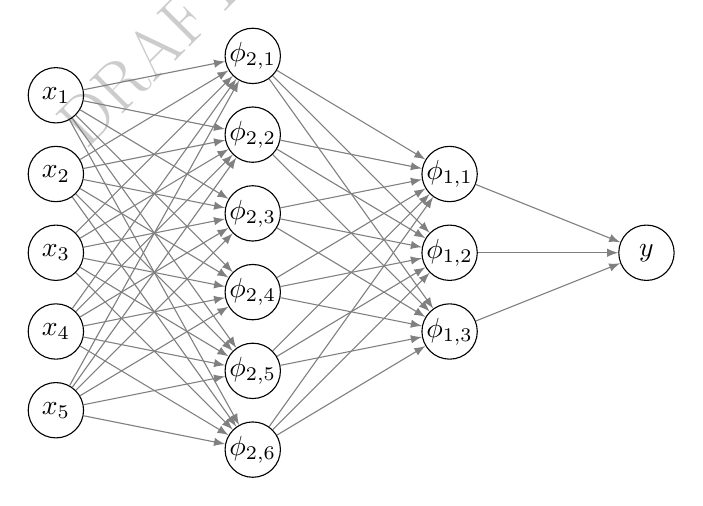
\begin{tikzpicture}[scale=0.5, node distance=2.5cm]
                \tikzstyle{neuron}=[
                    circle, draw, minimum size=20pt, inner sep=0pt]
                \tikzstyle{connector}=[->, arrows={-latex}, black!50]
                \foreach \name / \y in {1, ..., 5}
                    \node [neuron] (I-\name) at (0, -\y*2) {$x_\y$};

                \foreach \name / \y in {1, ..., 6}
                    \node [neuron] (P1-\name)
                        at (5, -\y*2 + 1) {$\phi_{2, \y}$};

                \foreach \name / \y in {1, ..., 3}
                    \node [neuron] (P2-\name)
                        at (10, -\y*2 - 2) {$\phi_{1, \y}$};

                \node [neuron] (y) at (15, -6) {$y$};

                \foreach \source in {1, ..., 5}
                    \foreach \dest in {1, ..., 6}
                        \path [connector] (I-\source) edge (P1-\dest);

                \foreach \source in {1, ..., 6}
                    \foreach \dest in {1, ..., 3}
                        \path [connector] (P1-\source) edge (P2-\dest);

                \foreach \source in {1, ..., 3}
                    \path [connector] (P2-\source) edge (y);
            \end{tikzpicture}
            \caption{A 2-layer neural network represented as a directed acyclic
                graph.}
            \label{fig:nn-as-dag}
        \end{figure}

    \subsection{Random Forests}
    \label{sec:random-forests}

        A \emph{decision tree} is a classifier that classifies by repeatedly
        dividing the feature space. Generating the tree proceeds as follows. The
        tree itself is a binary tree of decisions. The input space is split
        along one feature axis, giving two subtrees with one less dimension.
        This is then recursively applied to the subtrees until each leaf of the
        tree contains less than a given number of examples or until there are no
        more features to split on. The leaf nodes are then labelled with the
        most common label of the elements they contain.

        A \emph{random forest} is a classifier that uses an ensemble of decision
        trees to classify data points \citep{kon16}. A number of decision trees
        are generated, each with a different subset of features and inputs. This
        ensures that the decision trees are different. The random forest then
        classifies by having the decision trees vote on each label, with the
        most common vote being used as the prediction. The probability of this
        label being correct can be estimated as the percentage of decision trees
        in the ensemble that agree with the prediction.

        Random forests are nonlinear classifiers which are resistant to problems of feature scale. This makes them a good off-the-shelf classifier to apply to a generic classification problem.

\section{Feature Extraction from Images}
\label{sec:image-feature-extraction}
    
    For instances to be input to a classification model, they must be
    represented by vectors of features. Feature selection is generally a hard
    problem, but it may be straightforward if instances are simple vectors of
    measurements (such as in the breast cancer dataset described in Section
    \ref{sec:breast-dataset}). If the instances are provided in the form of
    images, however, feature selection becomes considerably harder.

    \subsection{The Na\"ive Approach}
    \label{sec:naive-approach-image-features}

        Images can be thought of as vectors of pixels, where the value of each
        pixel is treated as an independent feature. If the image is a colour
        image, then each channel (red, blue, and green) of each pixel can be
        treated as an independent feature. This is a very simple way to obtain
        features from images, with two considerable problems.

        \begin{figure}
            \centering
            \begin{subfigure}[t]{0.5\textwidth}
                \centering
                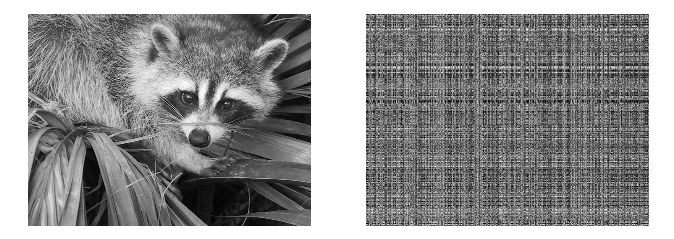
\includegraphics[width=\textwidth]{images/face.png}
            \end{subfigure}%
            ~
            \begin{subfigure}[t]{0.5\textwidth}
                \centering
                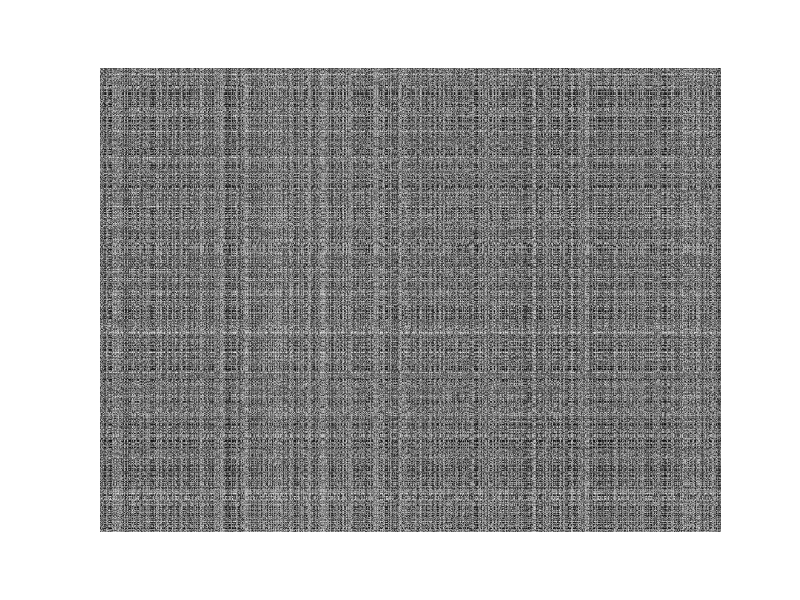
\includegraphics[width=\textwidth]{images/face_shuffled.png}
            \end{subfigure}
            \caption{If we ignore the location of pixels when interpreting an
                image as a vector, these two images have identical feature
                vectors, despite the left image clearly containing information
                not present in the right image.}
            \label{fig:shuffled-face}
        \end{figure}

        The first problem is that using pixels directly as independent features
        fails to accurately capture the image. The pixels are assumed
        independent when this is not the case --- neighbouring pixels are likely
        to be correlated, shapes and structure within the image introduce
        further correlations, and so on. If we are only looking at certain kinds
        of images, then the pixel location may also matter --- for example, we
        might have as inputs photographs of landscapes, where the sky tends to
        be at the top of the image --- and this information is also lost. These
        effects are shown in Figure \ref{fig:shuffled-face}. Finally, with
        independent pixels as features, trained models will be sensitive to
        small distortions or translations in the input \citep{lecun98}. In
        Section \ref{sec:convolutions}, we describe a common approach for
        resolving this problem.

        The second problem with this approach is that images tend to be large
        \citep{lecun98}. Taking each pixel as a feature leads to high
        dimensional feature spaces. This is not ideal as many algorithms perform
        poorly in high dimensional spaces. This can be resolved using
        \emph{pooling}, which we describe in Section \ref{sec:pooling}.

    \subsection{Pooling}
    \label{sec:pooling}

        \begin{figure}
            \centering
            \begin{subfigure}[t]{0.5\textwidth}
                \centering
                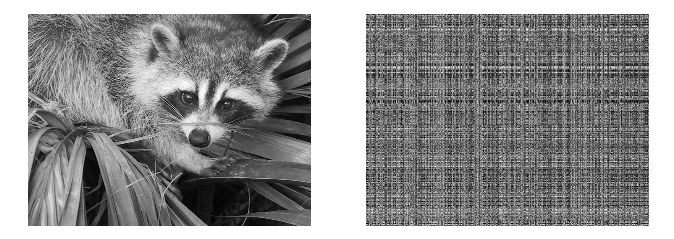
\includegraphics[width=\textwidth]{images/face.png}
                \caption{Original image.}
                \label{fig:pooling-face-original}
            \end{subfigure}%
            ~
            \begin{subfigure}[t]{0.5\textwidth}
                \centering
                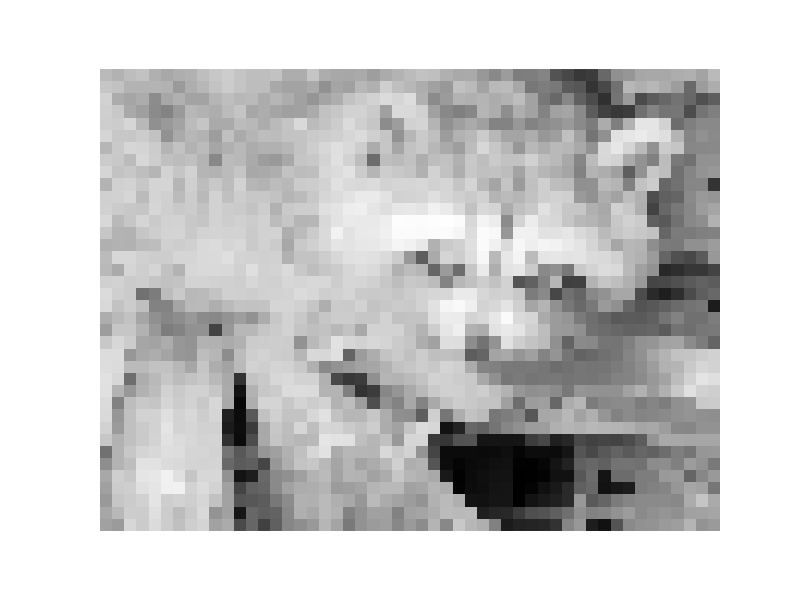
\includegraphics[width=\textwidth]{images/face_max_pooled.png}
                \caption{Max pooling.}
                \label{fig:pooling-face-max}
            \end{subfigure}
            \begin{subfigure}[t]{0.5\textwidth}
                \centering
                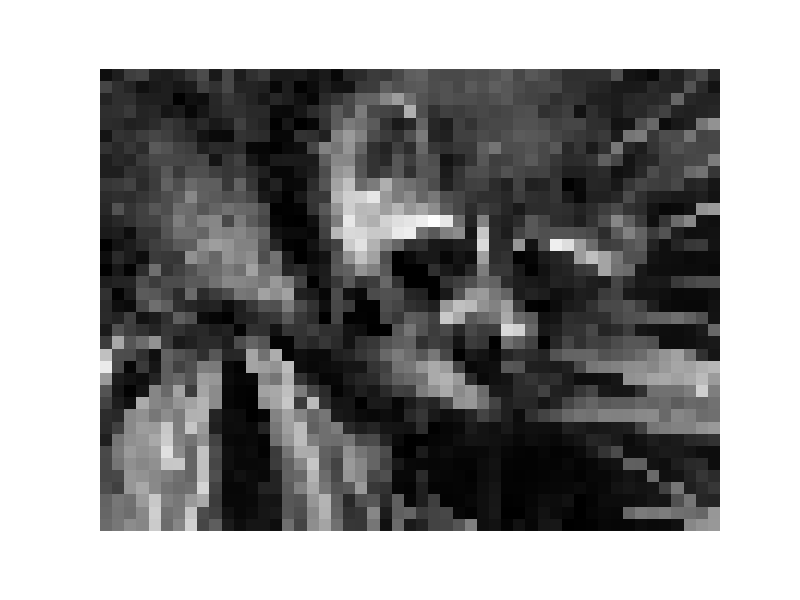
\includegraphics[width=\textwidth]{images/face_min_pooled.png}
                \caption{Min pooling.}
                \label{fig:pooling-face-min}
            \end{subfigure}%
            ~
            \begin{subfigure}[t]{0.5\textwidth}
                \centering
                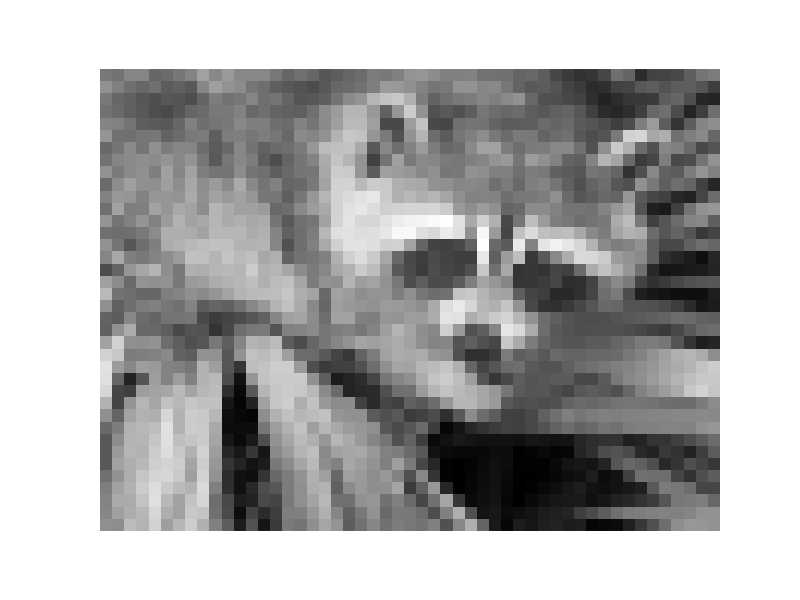
\includegraphics[width=\textwidth]
                    {images/face_average_pooled.png}
                \caption{Average pooling.}
                \label{fig:pooling-face-average}
            \end{subfigure}%
            \caption{Examples of max, min, and average pooling applied to an
                image.}
            \label{fig:pooling}
        \end{figure}

        Pooling is a class of operations that reduce the dimensionality of an
        image, parameterised by a \emph{pool size}\footnote{Another
        parameter is the \emph{stride}, $s$, which we ignore here for simplicity,
        setting $s = p$.}, $p$. Nonoverlapping $p \times p$ squares of pixels are
        condensed into one value, which becomes the corresponding pixel in the
        output. In this way, the size of the image is reduced from $m \times n$
        to $\frac{m}{p} \times \frac{n}{p}$. This results in both a smaller
        amount of data, and some amount of translation invariance when pooling
        is used in models like neural networks \citep{scherer10}.

        We are free to choose whatever aggregation operation we like to condense
        squares of pixels; common choices are $\max$ (called \emph{max pooling})
        and $\mbox{mean}$ (called \emph{average pooling}). Some pooling examples
        are shown in Figure \ref{fig:pooling}.

    \subsection{Convolutions}
    \label{sec:convolutions}

        \begin{figure}
            \centering
            \begin{subfigure}[t]{0.3\textwidth}
                \centering
                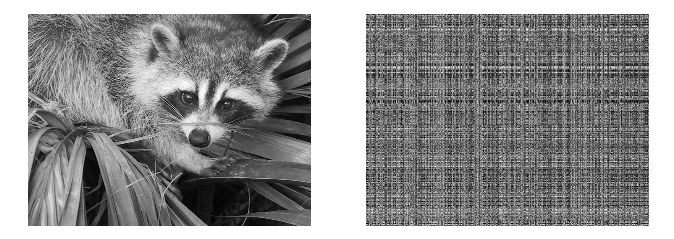
\includegraphics[width=\textwidth]{images/face.png}
                \caption{Original image.}
                \label{fig:convolution-face-original}
            \end{subfigure}%
            ~
            \begin{subfigure}[t]{0.3\textwidth}
                \centering
                
\includegraphics[width=\textwidth]
                    {images/convolutional_filter.png}
                \caption{Convolutional filter.}
                \label{fig:convolution-face-filter}
            \end{subfigure}%
            ~
            \begin{subfigure}[t]{0.3\textwidth}
                \centering
                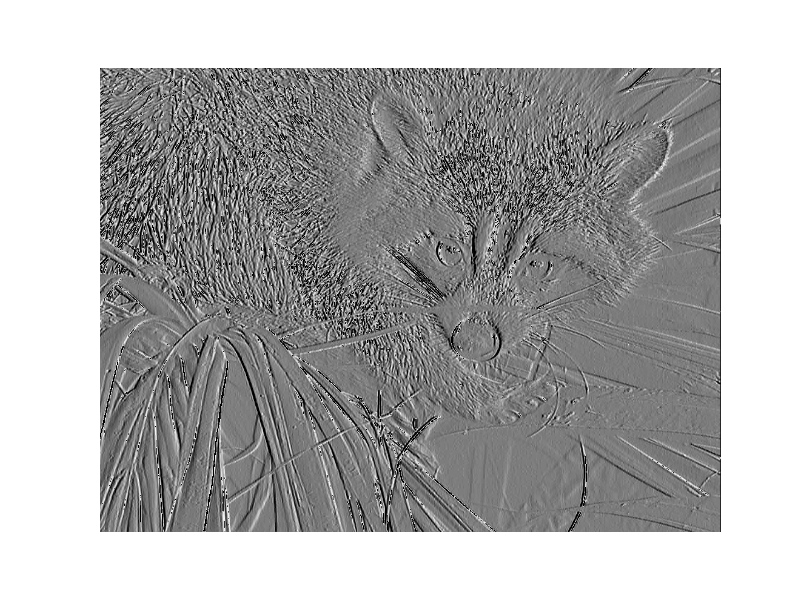
\includegraphics[width=\textwidth]{images/face_convolved.png}
                \caption{Convolved image.}
                \label{fig:convolution-face-convolved}
            \end{subfigure}
            \caption{Convolving an image with a $3 \times 3$ filter gives a new
                image. This filter acts as a kind of vertical edge detector.}
            \label{fig:convolved-face}
        \end{figure}

        A common way to make use of neighbourhood information in images is by
        using \emph{convolutions}. A convolution is an operation that transforms
        an image by applying an $n \times n$ \emph{filter} to each $n \times n$
        square of pixels. The filter is a matrix in $\mathbb{C}^{n \times n}$,
        and it is applied to a square of pixels by treating that square as a
        matrix, performing an elementwise multiplication between the filter
        matrix and the pixel matrix, and summing the result. Applying the filter
        to a square of pixels gives a single pixel value, so by applying the
        filter across the image, a new image is generated \citep{ludwig15}.

        One ambiguity is how to apply a filter to the edges of an image. There
        are multiple ways to resolve this. The most common method is to only
        apply the filter to squares of pixels fully contained within the image,
        making the output image smaller than the input. Another method is to
        apply the filter to the edges and assume that pixels outside the image
        have a constant value (usually 0), making the output image the same size
        as the input. These methods are commonly known as ``valid'' and ``same''
        respectively in libraries such as SciPy and Keras.

        The effect of a simple convolutional filter on an image is shown in
        Figure \ref{fig:convolved-face}, and an algorithm for performing a
        convolution is shown in Algorithm \ref{alg:convolution}.

        \begin{algorithm}
            \KwData{\\\quad{}An image $X \in \mathbb{R}^{m \times n}$%
                    \\\quad{}A filter $F \in \mathbb{C}^{d \times d}$}
            \KwResult{An image $\in
                \mathbb{R}^{(m - d + d \text{ mod } 2) \times
                            (n - d + d \text{ mod } 2)}$}

            Initialise output image $Y \in \mathbb{R}^{(m - d + d \text{ mod } 2) \times (n - d + d \text{ mod } 2)}$\;
            \For{$y \in \lfloor d/2 \rfloor, \dots, m - \lfloor d/2 \rfloor$}{
                \For{$x \in \lfloor d/2 \rfloor, \dots, n - \lfloor d/2 \rfloor$}{
                    $H \leftarrow$ $d \times d$ square of pixels centred on $(x, y)$\;
                    $Y_{y, x} \leftarrow (\vec 1^T (H \odot F) \vec 1) / (\vec 1^T F \vec 1)$\;
                }
            }

            \KwRet{$Y$}
            \caption{One method of performing a convolution. Here, we choose to
                use the ``valid'' method of handling edges, resulting in a
                smaller output than the input. $\odot$ is the elementwise
                matrix product.}
            \label{alg:convolution}
        \end{algorithm}

        By repeatedly applying convolutions and pooling, we can extract features
        from images that would not have been present using the na\"ive approach
        of Section \ref{sec:naive-approach-image-features}.

        \begin{itemize}
            \item CNNs are widely used now that we have a lot of data
            \item Robust and require minimal pre-processing (cite 21)
        \end{itemize}

    \subsection{Convolutional Neural Networks}
    \label{sec:convolutional-neural-networks}

        \begin{figure}
            \centering
            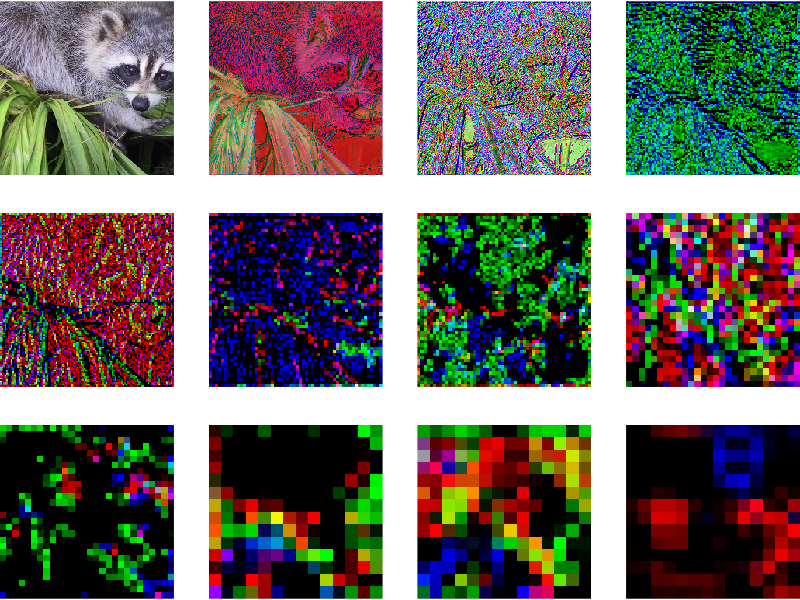
\includegraphics[width=\textwidth]{images/face_cnn.png}
            \caption{A convolutional neural network applied to the top-left
                image. The other images are the outputs of intermediate
                convolutional layers of the neural network, from left to right,
                top to bottom. Colours represent convolutions with different
                filters. The output, bottom-right, is a higher-level
                representation of the input image, and its values can be used
                as inputs for classification. This figure uses
                \citeauthor{baraldi15}'s implementation of the VGG-16 CNN
                \citep{simoyan14}.}
            \label{fig:face-cnn}
        \end{figure}

        While convolutions are needed to extract features from our images, there
        are no convolutions that work well in general. Convolutions must be
        chosen on a domain-dependent basis. This raises the question: What
        convolutions should we choose?

        One way to answer this question is simply to not choose at all, and
        then learn the appropriate convolutions as part of a larger
        classification model. This gives rise to the concept of a
        \emph{convolutional neural network} (CNN). A CNN is a neural network
        with layers that convolve their inputs and layers that pool their
        inputs, called \emph{convolutional layers} and \emph{pooling layers},
        respectively. Convolutional layers may contain any number of separate
        filters. They are generally interspersed with pooling layers. The final
        layers of the CNN are usually dense layers. Additionally, CNNs introduce
        some amount of translation invariance into their outputs, since the same
        filters are applied across the image \citep{lecun98}.

        CNNs can be used for feature extraction from images. As input, they
        take images to extract features from, and they are tasked with mapping
        these to some meaningful value or the intended output of the greater
        classification problem. The convolutional and pooling layers can then
        be isolated, forming a network that extracts features from images. An
        example of a convolutional neural network applied to an image is shown
        in Figure \ref{fig:face-cnn}.

\section{Crowdsourcing Labels}
\label{sec:crowdsourcing}

    For standard supervised learning tasks, the labels are generally provided by
    some \emph{expert}. We assume that the expert provides labels that are
    correct and accurately represent the groundtruth. More recently, however,
    many projects have \emph{crowdsourced} their labels: Non-expert people (the
    \emph{crowd}) volunteer or are paid to label data. The crowd may be sourced
    from websites like Amazon Mechanical Turk\footnote{\url{http://mturk.com}}
    where small amounts of money are paid on a per-label basis, or they may
    volunteer out of interest in the labelling project.

    Crowdsourcing allows us to quickly and cheaply label large amounts of data.
    This comes at the expense of objectivity and reliability --- since the crowd
    are necessarily non-experts, they do not have domain knowledge for the
    problem, and may not provide high-quality labels \citep{raykar10}. While we
    can try to reduce noise by requesting multiple labellers label each instance
    \citep{lin16, sheng08}, this does not address the fact that the data may be
    intrinsically hard to label, the labellers may be correlated, and some
    labellers may even be actively malicious \citep{yan10}. Some strategies to
    address these problems are described in Section \ref{sec:crowd-labels}.

    % The most obvious advantage of crowdsourcing is that crowds are able to
    % cheaply or quickly label large amounts of data simply because there are so
    % many people labelling. Crowds also allow us to gather labels on a wide
    % range of data

    The form of crowdsourcing we are interested in for this thesis is
    \emph{citizen science}, as this is form of crowdsourcing that the Radio
    Galaxy Zoo (Section \ref{sec:radio-galaxy-zoo}) uses. Citizen science is
    ``scientific work undertaken by members of the general public''
    \citep{oed-citizenscience, marshall15}, and has recently come to refer
    mainly to websites that allow non-experts to label scientific data. A
    notable example of citizen science is the Galaxy Zoo project
    \citep{lintott08}, which aims to identify morpologies of galaxies from the
    Sloan Digital Sky Survey. Galaxy Zoo has gathered tens of millions of labels
    for nearly $9 \times 10^5$ galaxies from over $8 \times 10^4$ volunteers
    \citep{lintott11}, and the data collected have been used in 48 publications
    so far\footnote{\url{https://www.zooniverse.org/about/publications}}. Many
    other citizen science projects have been hosted on the Galaxy Zoo's
    platform, Zooniverse\footnote{\url{http://zooniverse.org}}, from further
    astronomical studies like the Radio Galaxy Zoo \citep{banfield15} (Section
    \ref{sec:radio-galaxy-zoo}), which itself has labelled over $10^5$ radio
    sources from two radio surveys; to ecological studies like Snapshot
    Serengeti \citep{swanson15}, which has classified nearly 11 million camera
    trap images from Serengeti National Park.

    % Crowdsourcing is not without downsides. Since the crowd necessarily
    % consists of non-experts, there is no longer any guarantee that labels are
    % correct --- indeed, for the Radio Galaxy Zoo, balanced accuracy of
    % individual labellers varies from 40--100\%, with an average of 71\%.
    % Additionally, labels from different labellers may be correlated, different
    % labellers may be better skilled at labelling different kinds of examples,
    % some examples may be intrinsically hard for non-experts to label, and
    % labellers may even be actively malicious in giving incorrect labels
    % \citep{yan11}.

\section{Simulating a Crowd Labelling Task}
\label{sec:crowd-simulation}

    The crowd is inherently unpredictable. This makes it difficult to test
    methods for crowd learning, since there may be biases in existing
    crowd-labelled datasets, and we want our experiments to be both accurate and
    reproducible. To mitigate this problem, we instead simulate a crowd
    labelling task based on a dataset with known groundtruth. In this section,
    we describe our method for simulating a crowd labelling task, which we will
    later employ to test methods in Section \ref{sec:crowd-labels}. As part of
    this thesis, we have also implemented this simulation in Python. The
    implemention is described in Appendix \ref{sec:crowdastro-util}.

    \subsection{The Breast Cancer Wisconsin Dataset}
    \label{sec:breast-dataset}

        % This page formats really awfully due to the algorithm underneath.
        \raggedbottom

        The breast cancer Wisconsin dataset, first used by
        \citeauthor{wolberg90}, presents a classification task commonly used for
        testing classification methods. The dataset can be obtained from the UCI
        Machine Learning Repository \citep{lichman13}
        \footnote{\url{https://archive.ics.uci.edu/ml/%
                       datasets/Breast+Cancer+Wisconsin+\%28Original\%29}}.
        The classification task is, given medical observations of a patient,
        determine if their cancer is benign or malignant. Each instance is a
        10-dimensional feature vector, and there are 699 instances. There is
        some missing data, which we chose to set to 0.

    \subsection{Simulated Labeller Representation}
    \label{sec:simulated-labellers}

        We simulate $T$ labellers. Each labeller is indexed by a number $t$. The
        $t$-th labeller is represented by their \emph{sensitivity} (or \emph{true
        positive rate}) $\alpha_t$, and their \emph{specificity} (or \emph{true
        negative rate}) $\beta_t$, i.e.
        \begin{align*}
            \alpha_t &= p(y_t = 1 \mid z = 1)\\
            \beta_t &= p(y_t = 0 \mid z = 0)
        \end{align*}
        where $y_t$ is the label assigned by the $t$-th labeller to an instance
        with groundtruth $z$.

    \subsection{Obtaining the Simulated Labels}
    \label{sec:obtaining-simulated-labels}

        To generate crowd labels from our $T$ simulated labellers for a dataset
        with $N$ instances, we follow Algorithm \ref{alg:simulated-crowd}.

        \begin{algorithm}[H]
            \KwData{\\\quad{}A set of groundtruth labels $\{z_1, \dots, z_N\}$\\\quad{}A set of labellers $\{(\alpha_1, \beta_1), \dots, (\alpha_T, \beta_T)\}$.}
            \KwResult{A set of crowd labels $\{y_{1, 1}, \dots, y_{T, N}\}$.}

            \For{$i \in 1, \dots, N$}{
                \For{$t \in 1, \dots, T$}{
                    \eIf{$z_i = 1$}{
                        \WithProb{$\alpha_t$}{
                            $y_{t, i} \leftarrow 1$\;
                        }
                        \Else{
                            $y_{t, i} \leftarrow 0$\;
                        }
                    }{
                        \WithProb{$\beta_t$}{
                            $y_{t, i} \leftarrow 0$\;
                        }
                        \Else{
                            $y_{t, i} \leftarrow 1$\;
                        }
                    }
                }
            }
            \KwRet{$\{y_{1, 1}, \dots, y_{T, N}\}$}
            \caption{Simulating a crowd labelling task.}
            \label{alg:simulated-crowd}
        \end{algorithm}

\section{Utilising Crowd Labels}
\label{sec:crowd-labels}

    % There's kind of two things going on here - using multiple labels, and
    % using labels where the groundtruth doesn't exist. I should write about
    % that.

    A common method to combat label noise in crowd learning scenarios is to
    request multiple labels from the crowd for each data point.  There is some
    basis in the literature for such redundancy, with \citet{sheng08} showing
    that repeated labelling may improve label and model quality, though
    \citet{lin14} show that this is not always the case and results depend on
    the level and kind of label noise.

    Nevertheless, this approach is used in existing citizen science projects
    such as Galaxy Zoo \citep{lintott08} and Radio Galaxy Zoo
    \citep{banfield15}, both of which request 20 crowd labels for each instance.

    This raises the question of how best to make use of multiple labels to train
    classification models. In this section, we look at some methods that
    directly learn a model from multiple noisy labels, as well as some methods
    of aggregating the labels to obtain individual labels with (ideally) lower
    noise.

    \subsection{Majority Vote}
    \label{sec:majority-vote}

        One way to reduce label noise is to allow multiple labellers to label
        the same examples, and then for each example take the \emph{majority
        vote} to find a ``consensus'' label. If the label provided by the $t$-th
        labeller is denoted $y_t$ and there are $T$ labellers, then the
        consensus label is given by
        \begin{equation*}
            y = \begin{cases}
                1 & \frac{1}{T} \sum_{t = 1}^T y_t > 0.5\\
                0 & \frac{1}{T} \sum_{t = 1}^T y_t < 0.5\\
            \end{cases}
        \end{equation*}
        with the remaining case decided evenly at random \citep{raykar10}.

        The idea is that the majority of labels are correct, so with
        sufficiently large amounts of relabelling we expect the label noise to
        be reduced. How large ``sufficiently large'' is is unclear and
        domain-dependent, and is outside the scope of this thesis, though
        \citet{sheng08} and \citet{lin16} provide some information on how to
        choose relabelling rates. Of course, this fails in situations where the
        majority of labellers are not correct, which may be due to intrinsic
        difficulty or malicious labelling, or where there is no clear majority.

        One simple improvement to majority vote is to weight labels by the
        accuracy of the associated labeller, computing these accuracies based on
        some known groundtruth for a subset of the data. However, this requires
        access to the groundtruth for a subset of data, which is not available
        in general.

    \subsection{Raykar et al. Model}
    \label{sec:raykar}

        One way to learn from crowdsourced labels when no groundtruth is
        available is to jointly model both the reliability of each labeller (the
        \emph{labeller model}) and the groundtruth itself (the
        \emph{classification model}). \citet{raykar10} propose such a joint
        model, which we now describe.

        The accuracy of the $t$-th labeller is modelled by the sensitivity
        $\alpha_t$ and the specificity $\beta_t$, as described in Section
        \ref{sec:simulated-labellers}. This model assumes that labeller
        reliability is independent of the example $x$, but dependent on the
        groundtruth label $z$. Note that under this model, the probability that
        labeller $t$ will assign a given label to a positive example is given by
        \begin{equation*}
            p(y_t \mid z = 1, \alpha_t) =
                (\alpha_t)^{y_t} (1 - \alpha_t)^{1 - y_t}
        \end{equation*}
        and the probability that they will assign a given label to a negative
        example is given by
        \begin{equation*}
            p(y_t \mid z = 0, \beta_t) =
                (\beta_t)^{1 - y_t} (1 - \beta_t)^{y_t}.
        \end{equation*}
        For ease of notation, let $\vec \alpha = (\alpha_1, \dots, \alpha_t)$
        and $\vec \beta = (\beta_1, \dots, \beta_t)$.

        With this method, the classification model can be any classifier.
        \citeauthor{raykar10} choose to use logistic regression, i.e.
        \begin{equation}
            \label{eq:raykar-logreg}
            p(z = 1 \mid \vec x, \vec w) = \sigma(\vec w^T \vec x).
        \end{equation}

        The model parameters $\vec \theta = \{\vec w, \vec \alpha, \vec \beta\}$
        can be found by maximising the likelihood. Under the assumption that
        examples are independently sampled and labellers are independent, the
        likelihood is given by
        \begin{align*}
            p(\mathcal D \mid \vec \theta) &=
                \prod_{i = 1}^N
                    \prod_{t = 1}^T
                        p(y_{t, i} \mid \vec x_i, \vec w, \alpha_t, \beta_t)\\
            &\begin{aligned}=
                \prod_{i = 1}^N
                    \prod_{t = 1}^T
                        &\bigg[p(y_{t, i} \mid z_i = 1, \alpha_t)
                            p(z_i = 1 \mid \vec x_i, \vec w)\\
                        &+ p(y_{t, i} \mid z_i = 0, \beta_t)
                            p(z_i = 0 \mid \vec x_i, \vec w)\bigg].
             \end{aligned}
        \end{align*}
        Since there are unknown values $z$, the maximum likelihood problem must
        be solved using expectation-maximisation. This has closed-form solutions
        for $\vec \alpha$ (Equation \ref{eq:raykar-alpha}) and $\vec \beta$
        (Equation \ref{eq:raykar-beta}), but gradient methods must be used for
        finding $\vec w$.

        $\mu_i$ is initialised with majority vote, i.e.
        \begin{equation*}
            \mu_i = \frac{1}{T} \sum_{t = 1}^T y_{t, i}.
        \end{equation*}
        The expectation step requires us to compute
        \begin{align*}
            a_i &= \prod_{t = 1}^T
                (\alpha_t)^{y_{t, i}} (1 - \alpha_t)^{1 - y_{t, i}}\\
            b_i &= \prod_{t = 1}^T
                (\beta_t)^{1 - y_{t, i}} (1 - \beta_t)^{y_{t, i}}\\
            \mu_i &\propto
                \frac{a_i \sigma(\vec w^T \vec x_i)}
                     {a_i \sigma(\vec w^T \vec x_i) +
                      b_i (1 - \sigma(\vec w^T \vec x_i))}.
        \end{align*}
        The maximisation step requires us to compute
        \begin{align}
            \label{eq:raykar-alpha}
            \alpha_t &= \frac{\sum_{i = 1}^N \mu_i y_{t, i}}
                             {\sum_{i = 1}^N \mu_i}\\
            \label{eq:raykar-beta}
            \beta_t &= \frac{\sum_{i = 1}^N (1 - \mu_i) (1 - y_{t, i})}
                            {\sum_{i = 1}^N (1 - \mu_i)}
        \end{align}
        and find the $\vec w$ that maximises the likelihood using gradient
        methods. In my implementation of this algorithm, I initialised $\vec w$
        using logistic regression trained on the majority vote, and then used
        the old $\vec w$ to initialise each subsequent maximisation step.

        As part of this thesis, we have produced an open source implementation
        of this algorithm, described in Appendix \ref{sec:crowdastro-raykar}. We
        then performed a series of experiments using this implementation, which
        are detailed here.

        \subsubsection{Testing the Raykar Classifier}

            \begin{figure}
                \centering
                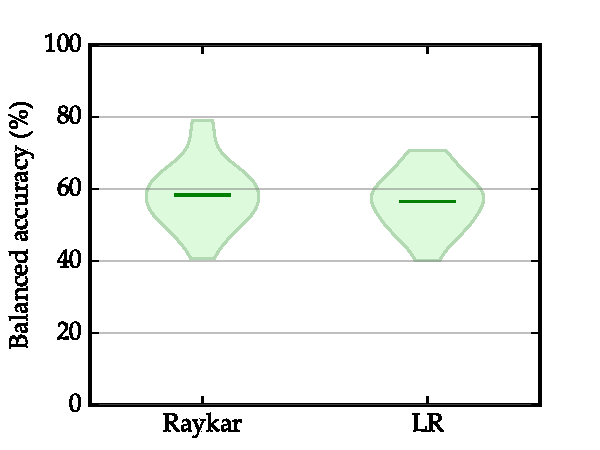
\includegraphics[height=0.3\textheight]
                    {images/experiments/raykar.pdf}
                \caption{Performance of the \citeauthor{raykar10} classifier
                    against logistic regression (LR) on a simulated crowd
                    labelling of the breast cancer dataset \citep{wolberg90}.}
                \label{fig:raykar}
            \end{figure}

            We first used the implementation to perform a simple, simulated
            crowd labelling problem. Five simulated labellers were assigned true
            positive and false positive rates uniformly distributed in the range
            $[0.25, 0.75]$. Each simulated labeller labelled 50\% of the breast
            cancer dataset (Section \ref{sec:breast-dataset}). Random samples of
            75\% of the examples were drawn 20 times and used to train both the
            \citeauthor{raykar10} classifier and a logistic regression
            classifier (using majority vote for the labels). To help find a good
            set of parameters, the \citeauthor{raykar10} classifier was
            retrained 5 times with random initial conditions, and the classifier
            attaining the highest likelihood was selected. Both logistic
            regression and \citeauthor{raykar10} classifiers were tested against
            the groundtruth of the remaining 25\%. The results are plotted in
            Figure \ref{fig:raykar}. The Raykar classifier attained a balanced
            accuracy of $(58 \pm 8)\%$ and the logistic regression classifier
            attained a balanced accuracy of $(56
            \pm 8)\%$.

            From this experiment, we can see that the \citeauthor{raykar10}
            algorithm performs comparably to logistic regression, even under
            high noise. However, training a logistic regression classifier on
            the majority vote is far simpler and faster, even in an idealised
            scenario where labeller noise is exactly modelled by the
            \citeauthor{raykar10} model. This may be an artefact of the
            expectation-maximisation algorithm, which is never guaranteed to
            converge to a global maximum. If so, then increasing the number of
            random restarts may improve results, at the cost of increased
            training time.

        \subsubsection{The Effect of Class Imbalance}

            \begin{figure}
                \centering
                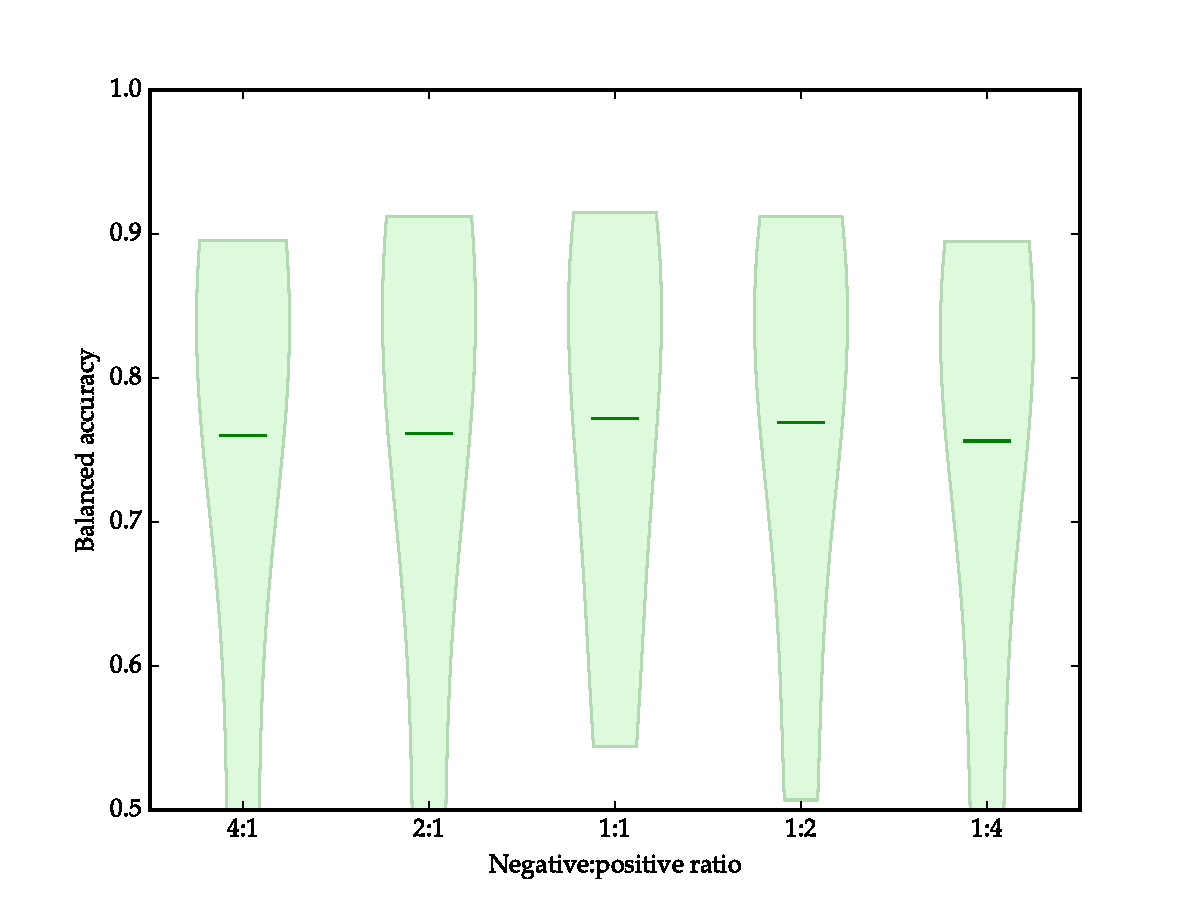
\includegraphics[width=0.8\textwidth]
                    {images/experiments/raykar_class_balance_ba}
                \caption{Performance of the \citeauthor{raykar10} classifier on
                    a simulated labelling problem with different class
                    imbalance.}
                \label{fig:raykar-class-balance-ba}
            \end{figure}

            \begin{figure}
                \centering
                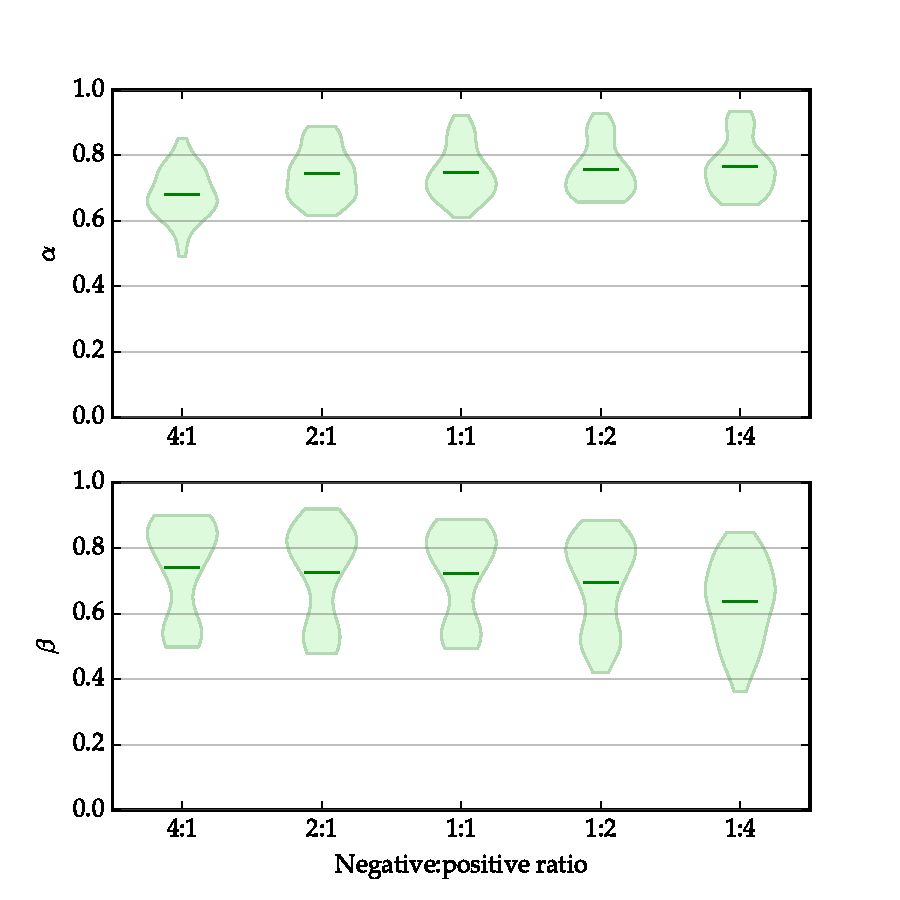
\includegraphics[width=0.8\textwidth]
                    {images/experiments/raykar_class_balance}
                \caption{Output $\alpha$ and $\beta$ values of the
                    \citeauthor{raykar10} classifier on a simulated labelling
                    problem with different class imbalance.}
                \label{fig:raykar-class-balance-ab}
            \end{figure}

            The second experiment tested the effect of class imbalance on the
            resulting balanced accuracy of the classifier, as well as on the
            predicted $\alpha$ and $\beta$ for each labeller. We used
            scikit-learn's \texttt{sklearn.datasets.make\_classification}
            function \citep{scikit-learn} to generate datasets with
            5-dimensional features (of which 3 were informative, and 2 were
            redundant) with a class separation of 1 and 1\% of true labels
            randomly flipped. We generated five datasets, each with 1000
            examples, with different ratios of negative to positive examples.
            The ratios were $4:1$, $2:1$, $1:1$, $1:2$, and $1:4$. We then
            simulated a crowd labelling task as in Section
            \ref{sec:crowd-simulation}, assigning 10 labellers true positive and
            false positive rates uniformly at random in the interval $[0.5,
            0.9]$ and allowing them to ``label'' the examples. The same
            labellers were used across all trials and datasets. We ran the
            \citeauthor{raykar10} algorithm on each dataset and recorded the
            balanced accuracy and output $\alpha$ and $\beta$ values for each
            trial and dataset. We repeated this experiment 5 times. The
            resulting balanced accuracies are plotted against the ratios of
            negative to positive examples in Figure
            \ref{fig:raykar-class-balance-ba}, and the estimated $\alpha$ and
            $\beta$ values are plotted against the ratios in Figure
            \ref{fig:raykar-class-balance-ab}.

            The balanced accuracy is similarly distributed across all trials,
            with a slight decrease as classes grow more unbalanced. The
            estimated $\alpha$ and $\beta$ values are also similar across all
            trials. This shows that our implementation of the
            \citeauthor{raykar10} algorithm is not sensitive to class imbalance.

        \subsubsection{The Effect of Label Noise}

            \begin{figure}
                \centering
                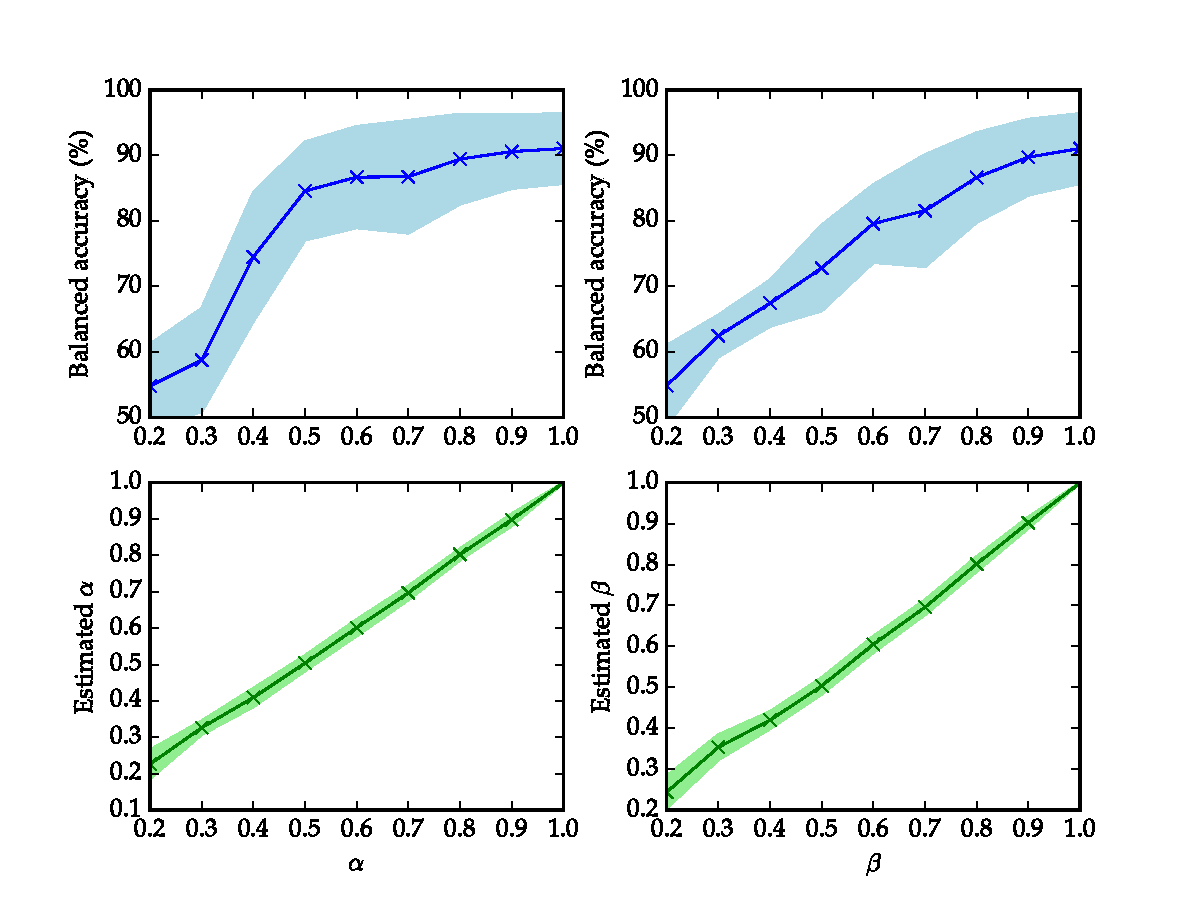
\includegraphics[width=\textwidth]
                    {images/experiments/raykar_noise}
                \caption{Output $\alpha$, $\beta$, and balanced accuracy of the
                    \citeauthor{raykar10} classifier on a simulated labelling
                    problem with different amounts of label noise. ``Estimated
                    $\alpha$'' refers to the value of $\alpha$ output by the
                    algorithm, and $\alpha$ refers to the groundtruth. Filled
                    areas represent the standard deviation of multiple
                    measurements.}
                \label{fig:raykar-noise}
            \end{figure}

            The final experiment was to determine the effect of label noise on
            the performance and output of the algorithm. 10 labellers were
            simulated with $\alpha$ ranging from $0.2$ to $1.0$ and $\beta$
            fixed at $1.0$. A dataset was generated as for the previous
            experiment (but with balanced classes), the labellers were tasked
            with labelling this dataset, and the labels were used to train the
            algorithm. The balanced accuracy and $\alpha$ values were recorded.
            This experiment was repeated $5$ times, and repeated again with
            $\beta$ replacing $\alpha$. The results are shown in Figure
            \ref{fig:raykar-noise}.

            As expected, the balanced accuracy increases as label noise
            decreases, and the output $\alpha$ and $\beta$ closely match the
            true values. This shows that our implementation of the
            \citeauthor{raykar10} algorithm is able to recover the noise
            parameters of our simulated labellers.

    \subsection{Yan et al. Model}
    \label{sec:yan}

        A similar approach is described by \citet{yan10}, again jointly learning
        the groundtruth and labeller models. Unlike \citeauthor{raykar10}, the
        \citeauthor{yan10} labeller model is data-dependent. The accuracy of the
        $t$-th labeller is modelled by a Bernoulli distribution of $\eta_t(\vec
        x)$, parametrised as a logistic regression function $\eta_t(\vec x) =
        \sigma(\vec \omega_t^T \vec x + \gamma_t)$. The labeller model is thus
        \begin{equation*}
            p(y_t \mid \vec x, z, \vec \omega_t, \gamma_t) =
                \eta_t(\vec x)^{1 - |y_t - z|} (1 - \eta_t(\vec x))^{|y_t - z|}.
        \end{equation*}
        For ease of notation, let $\Omega = (\vec \omega_1^T, \dots,
        \vec \omega_T^T)$ and let $\vec \gamma = (\gamma_1, \dots, \gamma_T)$.
        This model can be obtained from the \citeauthor{raykar10} model by
        requiring $\alpha_t = \beta_t = \eta_t(\vec x)$ and allowing these
        parameters be data-dependent.

        As with \citeauthor{raykar10}, the classification model can be any
        classifier and \citeauthor{yan10} choose to use logistic regression
        (Equation \ref{eq:raykar-logreg}). The parameters $\vec \theta =
        \{\Omega, \vec \gamma, \vec w\}$ can be found by maximising the
        likelihood with expectation-maximisation. Under the assumptions that
        examples are independently sampled and that the labellers are
        independent, the likelihood is given by
        \begin{align*}
            p(\mathcal D \mid \vec \theta)
                &= \prod_{i = 1}^N \prod_{t = 1}^T
                    p(y_{t, i} \mid \vec x_i, \vec w, \Omega, \vec \gamma)\\
                &= \prod_{i = 1}^N \prod_{t = 1}^T \sum_{z = 0}^1
                    p(y_t \mid \vec x_i, z, \vec \omega_t, \gamma_t)
                    p(z \mid \vec x_i, \vec w).
        \end{align*}
        The expectation step requires us to compute
        \[
            \mu_i \propto \prod_{t = 1}^{T}
                p(y_{t, i} \mid \vec x_i, z_i = 1, \vec \omega_t, \gamma_t)
                p(z_i = 1 \mid \vec x_i, \vec w).
        \]
        The maximisation step requires us to maximise
        \begin{equation*}
            \sum_{i = 1}^N \sum_{t = 1}^T \sum_{z_i = 0}^1
                p(z_i \mid \vec x_i, \vec w) (
                    \log p(y_{t, i} \mid \vec x_i, z, \vec \omega_t, \gamma_t) +
                    \log p(z \mid \vec x_i, \vec w))
        \end{equation*}
        with respect to $\vec w, \Omega,$ and $\vec \gamma$, where $p(z_i \mid
        \vec x_i, \vec w)$ is fixed to use the previous value of $\vec w$.

        As part of this thesis, we have produced an open source implementation
        of this algorithm, described in Appendix \ref{sec:crowdastro-yan}. After
        the algorithm was implemented, we found it to be considerably slower
        than the \citeauthor{raykar10} algorithm, so we do not use it later in
        this thesis. Its inclusion in this thesis is to show that the
        expectation-maximisation approach can be extended by choice of labeller
        model.

        \begin{figure}
            \centering
            \begin{subfigure}{\textwidth}
                \centering
                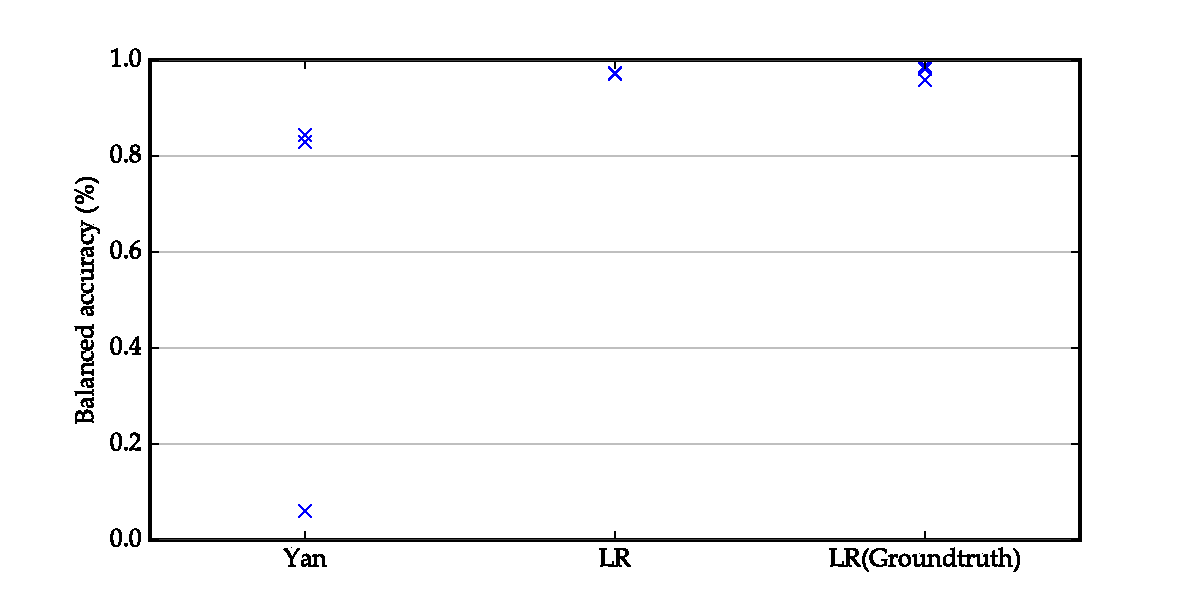
\includegraphics[width=0.9\textwidth]
                    {images/experiments/yan_25pc_noise.pdf}
                \caption{$\upsilon = 75\%$}
                \label{fig:yan-experiment-low-noise}
            \end{subfigure}
            \begin{subfigure}{\textwidth}
                \centering
                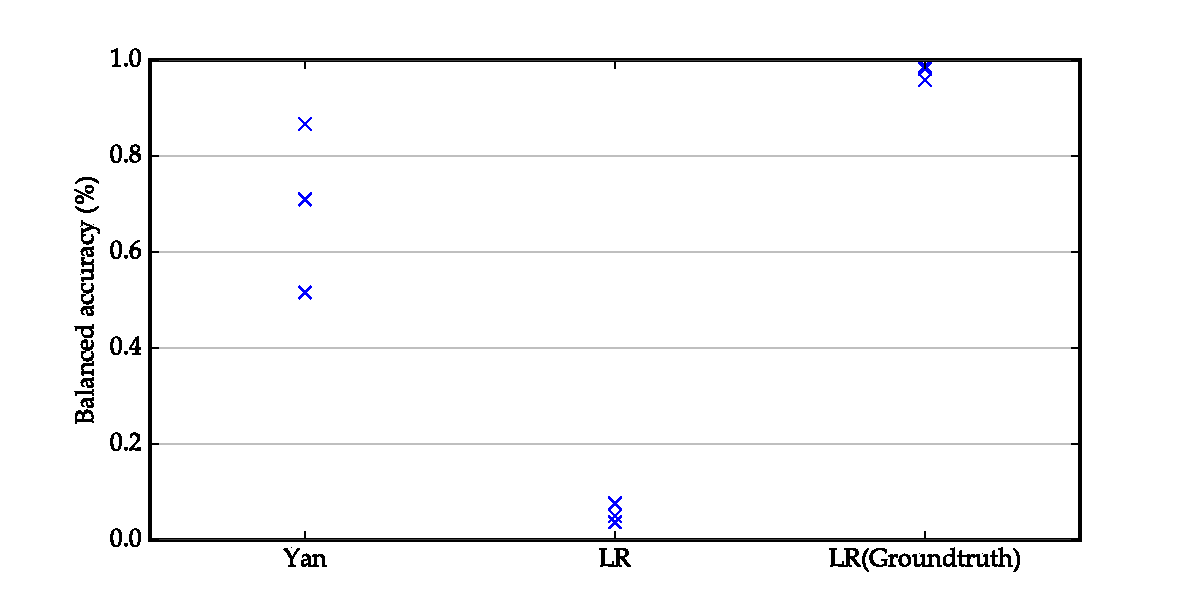
\includegraphics[width=0.9\textwidth]
                    {images/experiments/yan_75pc_noise.pdf}
                \caption{$\upsilon = 25\%$}
                \label{fig:yan-experiment-high-noise}
            \end{subfigure}
            \caption{\citeauthor{yan10} algorithm compared with logistic
                regression trained on the majority vote (LR) and logistic
                regression trained on the groundtruth (LR(Groundtruth)).
                Labellers have an accuracy of $\upsilon$ when not in
                their cluster of expertise.}
        \end{figure}

        The \citeauthor{yan10} algorithm is good for modelling labellers with
        highly feature-dependent noise. To test the algorithm, we employed it on
        the breast cancer Wisconsin dataset (Section \ref{sec:breast-dataset}),
        but using a different simulation of labellers to that used for the
        \citeauthor{raykar10} tests of Section \ref{sec:raykar}. While the
        method for generating simulated crowd labels was similar, the labeller
        model differed to show the ability of the \citeauthor{yan10} model to
        handle feature-dependent noise. Instead of using two values $\alpha$ and
        $\beta$ to describe each labeller, we clustered the data and assigned
        each labeller one cluster. The labeller had $100\%$ accuracy for that
        cluster, and a fixed accuracy $\upsilon$ for all other clusters, giving
        each labeller a ``cluster of expertise''. We tested with low noise
        ($\upsilon = 0.75$) and high noise ($\upsilon = 0.25$). The results are
        compared with logistic regression trained on the majority vote and
        logistic regression trained on the groundtruth in Figure
        \ref{fig:yan-experiment-low-noise} and Figure
        \ref{fig:yan-experiment-high-noise} for low and high noise,
        respectively.

        From these plots, we can tell that with low noise, logistic regression
        is able to learn a high quality model from the majority vote, while the
        \citeauthor{yan10} model performs more poorly. While it is possible for
        the \citeauthor{yan10} model to reduce to logistic regression, this is
        evidently not guaranteed in practice. This may be due to the difficulty
        of the expectation-maximisation problem, which is never guaranteed to
        converge on a global maximum in general. When noise is high, however,
        the \citeauthor{yan10} algorithm considerably outperforms logistic
        regression, indicating that in situations with high, feature-dependent
        noise, the \citeauthor{yan10} algorithm may be a good choice of
        classification algorithm. However, this choice of labeller model may not
        be ideal with large numbers of labellers. There are $ND$ parameters, so
        the expectation-maximisation algorithm may converge considerably slower
        and the number of local minima may quickly increase with increasing
        numbers of labellers.

%!TEX root=thesis.tex

\chapter{Radio Cross-identification}
\label{cha:cross-identification}

  In this chapter, we develop a machine learning approach to the radio cross-%
  identification problem. First, we discuss different ways to train and use
  a classifier for the task, in particular framing the cross-identification
  problem as an object localisation problem. We then discuss the available
  training data and how we chose to process it. Finally, we present results
  against a dataset of expert labels, and compare these results to those found
  by other methods.

\section{Formalism}
\label{sec:cross-identification-formalism}

  We begin by restating the cross-identification problem (Section
  \ref{sec:radio-cross-identification}). When we look at the sky with radio
  telescopes, we see the radio emissions from the jets of AGNs. Given an image
  of these radio emissions, and possibly other images in other wavelengths, we
  want to locate the host galaxy containing the associated AGN. In general,
  there may be multiple hosts associated with one radio object (such as in
  Figure \ref{fig:two-hosts}), but we make the assumption that there is only
  one. This greatly simplifies the problem.

  \begin{figure}[!ht]
    \centering
    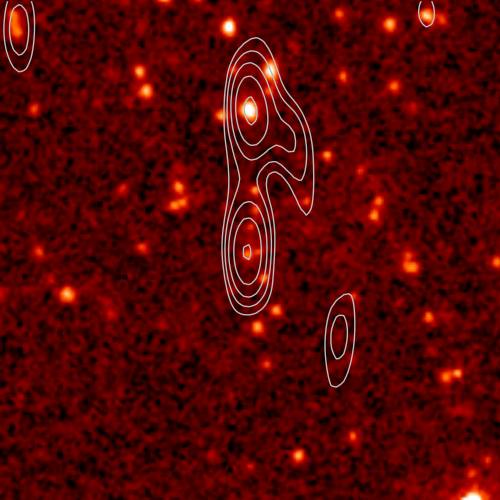
\includegraphics[width=0.5\textwidth]{images/CI0370C1_heatmap+contours.png}
    \caption{A radio object (ARG0003ra1) with two host galaxies. This radio
      object is actually two radio objects that have been incorrectly detected
      as one, and there is one host galaxy for each object.}
    \label{fig:two-hosts}
  \end{figure}

  \subsection{Cross-identification as Object Localisation}
  \label{sec:object-localisation}

    We can interpret cross-identification as an object localisation problem. As
    input, we have an image of the radio sky, and we want to locate a host
    galaxy in this image. A common way to find an object in an image is by using
    a sliding window. A fixed-size image patch centred on each pixel is taken as
    a representation of that pixel. This is then used as input to a
    classification model which outputs a probability for each pixel, with higher
    probabilities corresponding to higher likelihood of the object being located
    at that pixel. The pixel with the highest probability is considered the
    location of the object.

    This may be slow depending on the size of the image. One way to improve upon
    this approach is to first identify a small number of candidate locations,
    and then only examine patches around these locations. For the cross-%
    identification problem, we can use galaxy locations as candidate pixels,
    with galaxies found in infrared surveys such as WISE and SWIRE.
    Additionally, astronomical measurements such as magnitude are included in
    these surveys and these may be taken as additional features for each
    candidate pixel, giving more information to the classifier.

  \subsection{The Galaxy Classification Task}
  \label{sec:galaxy-classification-task}

% \section{Cross-identification as Binary Classification}
% \label{sec:framing-as-classification}

  This approach can be formalised as follows. Consider a set $\mathcal X$ of
  candidate host galaxies, and a radio object $r$ that we want to assign a
  host galaxy. Let $y : \mathcal X \to \{0, 1\}$ represent whether a given $x
  \in \mathcal X$ is the host galaxy associated with $r$. Under the assumption
  that a radio object has exactly one associated host galaxy, then there exists
  exactly one $x \in \mathcal X$ such that $y(x) = 1$, and for all other $x \in
  \mathcal X$, $y(x) = 0$. The cross-identification task then amounts to
  modelling $p(y(x) = 1 \mid x, r)$. Once this distribution is modelled, the
  host galaxy associated with $r$ is given by
  \begin{equation}
      \label{eq:cross-identification}
      \mbox{host}(r) = \underset{x}{\mbox{argmax}}\ p(y(x) = 1 \mid x, r).
  \end{equation}

  Ideally, $\mathcal X$ is the set of all galaxies. This is clearly
  intractable, so as an approximation we use a catalogue of infrared objects
  near the radio object of interest, taken from an infrared survey. We also
  make the assumption that the host galaxy is within $1'$ of the radio object
  --- while this doesn't hold in general, systems larger than $1'$ are rare and
  require human insight to discover \citep{banfield16}.

\section{Evaluating Performance Without Groundtruth}
  \label{sec:norris-as-groundtruth}

  In general, we do not have groundtruth for the cross-identification problem.
  While the groundtruth exists (a galaxy either has an AGN or does not), it is
  impossible for us to measure this accurately. Even expert catalogues, such as
  those provided by \citeauthor{norris06} (Section \ref{sec:norris}), are noisy
  --- \citep{norris06} estimate that their cross-identifications have a $9.02\%$
  false positive rate.
  
  Our primary source of labels for the classification task is the Radio Galaxy
  Zoo. These labels have been provided by non-experts, and as such are even more
  noisy. This leads to two problems: A classifier trained on the noisy labels
  may be inaccurate, and evaluating the performance of a trained classifier
  against noisy labels will not accurately reflect the true performance of the
  classifier. We address the former in Section \ref{sec:rgz-crowd-labels}, and
  the latter here.

  The obvious way to evaluate classifier performance without groundtruth is to
  aggregate the Radio Galaxy Zoo crowd labels in some way to approximate the
  groundtruth, and then use that for evaluation. While there are many ways that
  we could aggregate the labels (Section \ref{sec:rgz-crowd-labels}), these
  aggregates are \emph{not} the groundtruth and may still contain high noise. We
  want our classifier to be capable of finding the best approximation to the
  groundtruth, not to the noisy inputs, and evaluation should reflect that. We
  therefore cannot use aggregated crowd labels for evaluation.

  To attempt to mitigate this problem, we chose a test set with as little noise
  as possible by combining the \citeauthor{norris06} catalogue (Section
  \ref{sec:norris}) with the \citeauthor{fan15} catalogue (Section
  \ref{sec:fan}) to find all galaxies for which the two catalogues agree.
  Test sets were drawn from only these galaxies. This does mean that the test
  instances will be ``easier'' than a test set drawn from the entire data set,
  but any tests performed against these test sets should be more reliable than
  would otherwise be the case.

\section{Experiment Design}
\label{sec:experiment-design}

  To guide our classifier design, we needed to run experiments. This section
  describes the design and test sets used for the experiments that appear in the
  following sections.

  To generate the \citeauthor{norris06} and \citeauthor{fan15} label sets, we
  matched each location identified by \citeauthor{norris06} and
  \citeauthor{fan15} to the nearest candidate host in WISE. These galaxies were
  labelled $1$. All other candidate hosts were labelled $0$.

  We generated test sets by first finding all candidate hosts for which the
  \citeauthor{norris06} label and the \citeauthor{fan15} label agree. To
  generate a test set, we followed the following method:
  \begin{enumerate}
    \item Find all ATLAS objects where \citeauthor{norris06} and
    \citeauthor{fan15} agree on the labels of all galaxies within 1'.
    \item Draw randomly without replacement 50\% of the ATLAS objects.
    \item If a candidate host is within 1' of a drawn ATLAS object, add it to
    the test set.
  \end{enumerate}
  This method resulted in a test set with similar class distribution to the true
  data and no feature overlap between training objects and testing objects. We
  drew 10 test sets with this method.

  To train and test a method, we followed the following method:
  \begin{enumerate}
    \item Choose a test set.
    \item Add all candidate hosts not in this test set to the training set.
    \item Train the method using the selected training set.
    \item Evaluate performance with balanced accuracy against the test set.
    \item Repeat for all other test sets.
  \end{enumerate}
  We report the mean balanced accuracy and standard deviation.

\section{Feature Selection}
\label{sec:features}

  To train a machine learning method to solve the galaxy classification task,
  we must find a representation of galaxies in a feature space $\mathbb{R}^D$.
  In this section we describe and motivate our choice of galaxy features,
  extracted from both infrared and radio surveys.

  \subsection{Infrared Features}
  \label{sec:ir-features}

    \begin{figure}
      \centering
      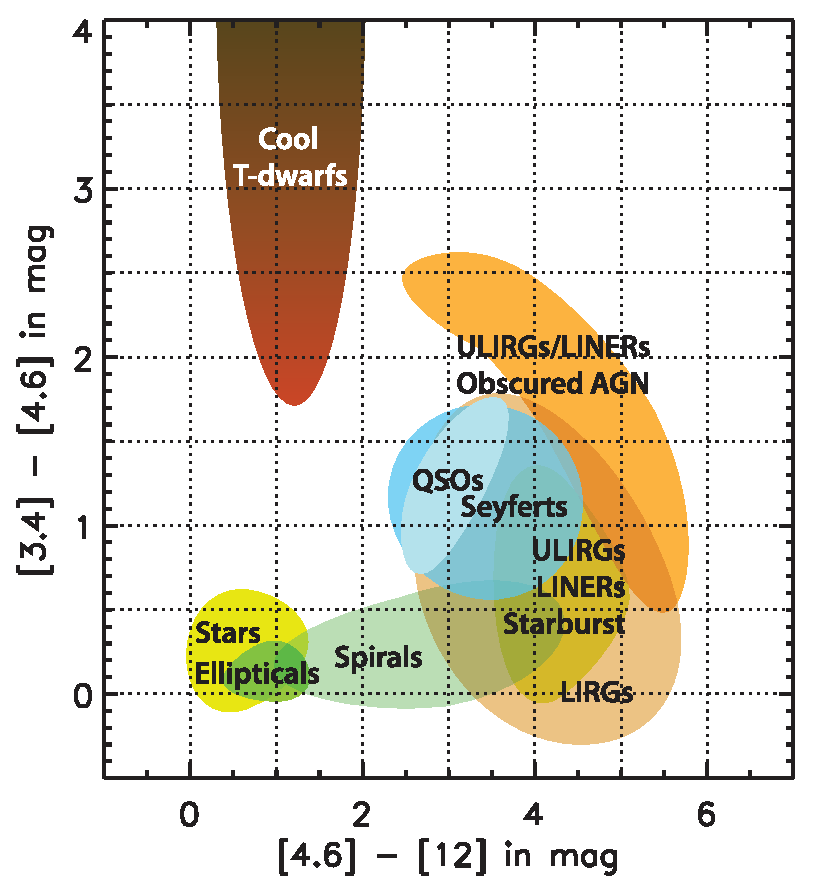
\includegraphics[width=0.5\textwidth]{images/wise_colour-colour}
      \caption{WISE colour-colour diagram showing the colours of various
        astronomical objects. The horizontal axis is $w2 - w3$ and the vertical
        axis is $w1 - w2$. Reproduced from \citep{wright10}.}
      \label{fig:wise-colour-colour}
    \end{figure}

    As described in Section \ref{sec:cross-identification-formalism}, we need
    candidate host galaxies from an infrared catalogue. We have two choices here
    --- the WISE catalogue (Section \ref{sec:wise}) and the SWIRE catalogue
    (Section \ref{sec:swire}). WISE is lower resolution and less sensitive, but
    is the survey that will be used to cross-identify EMU (Section
    \ref{sec:emu}) sources when they are available. SWIRE has higher
    resolution and sensitivity, and thus would give more accurate galaxies, but
    it does not cover the whole sky. Here, we describe our choice of features
    for both.

    For WISE, we chose to use all four WISE band magnitudes ($w1, w2, w3,$ and
    $w4$) as features. Since the features are magnitudes, they are on a
    logarithmic scale, and we found that in practice classification performance
    improved when the magnitudes were converted to their corresponding flux
    value. We performed this conversion with the formula
    \begin{equation}
      \label{eq:mag-to-flux}
      f = 10^{-0.4m}.
    \end{equation}
    This is the inverse of Equation \ref{eq:apparent-magnitude} with the flux in
    linear units of $f_{\text{Vega}}$ Jy.

    The ratios between infrared fluxes are indicators of physical galactic
    properties such as star formation and dust \todo{Find a source on this ---
    Probably the WISE paper wright10}. In practice, the $w1 - w2$ and $w2 - w3$
    ratios are most commonly used (such as in Figure
    \ref{fig:wise-colour-colour}), so we chose to use these ratios as features.
    Once again, we used a linear scale, computing the ratios using equation
    \ref{eq:magnitude-difference} and converting them to linear units with
    Equation \ref{eq:mag-to-flux}.

    Also available were the unprocessed infrared images captured in the survey.
    Under the assumption that the large scale infrared structure of a galaxy is
    unchanged by an AGN, we chose to ignore the images themselves and focus on
    features obtained from the catalogue. This greatly simplified feature
    selection with minimal expected impact on the classification performance.
    Future work may investigate the effectiveness of features extracted from
    infrared images on classification performance, but this is out of the scope
    of this thesis.

    SWIRE also contains colour information, but unlike WISE, the information is
    in the form of fluxes instead of magnitudes. This means that the flux
    information in the catalogue can be used as features directly. The ratios
    can also be used --- $3.6\ \mu\text{Jy} / 4.5\ \mu\text{Jy}$ and $4.5\
    \mu\text{Jy} / 5.8\ \mu\text{Jy}$ are the SWIRE equivalents of $w1 - w2$ and
    $w2 - w3$. Since SWIRE is higher resolution than WISE, the
    infrared images may contain more useful information and thus be useful for
    features, but this was not explored in this thesis.

    % The SWIRE catalogue (Section \ref{sec:swire}) also contains colour
    % information for each contained object, but only fluxes rather than
    % magnitudes. \todo{Read the SWIRE colour-colour diagram and continue this.}

    % Both WISE and SWIRE catalogues contain the positions of each object. The
    % distance from each object to the centre of the closest radio object is
    % used as a feature representing that object. This noticeably improves
    % classification performance \todo{make an experiment showing this, and
    % probably also showing that the other features are good}.

  \subsection{Radio Features}
  \label{sec:radio-features}

    While the infrared catalogues include measurements on individual galaxies,
    the ATLAS radio catalogue does not. This is because galaxies are not
    visible in radio, so while galaxies are directly represented in an infrared
    catalogue they are not in a radio catalogue. Galactic features must thus be
    extracted from the radio images directly. We chose to use a convolutional
    neural network, as described in Section \ref{sec:image-feature-extraction}.

    \subsubsection{Building a Model for Feature Extraction}
    \label{sec:feature-extraction-model}

      \begin{figure}[!ht]
         \centering
         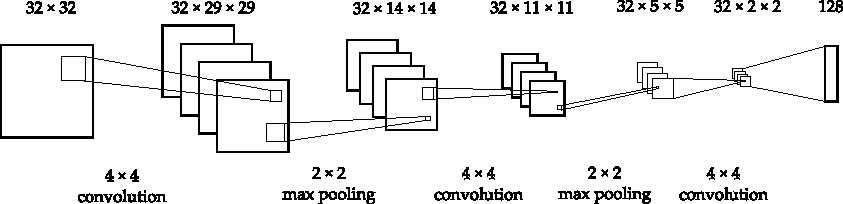
\includegraphics[width=\textwidth]{images/cnn_new.pdf}
         \caption{Convolutional neural network for radio feature extraction. The
           leftmost square represents the input image; the rightmost rectangle
           is the output.}
         \label{fig:radio-cnn}
       \end{figure}

      We chose to use a convolutional neural network (CNN) with three
      convolutional and max pooling layers, shown in Figure \ref{fig:radio-cnn}.
      This resulted in an 128-dimensional feature vector. For training this
      network, we added a 64-dimensional dense layer mapping to a 1-dimensional
      output. 10\% of ATLAS objects were selected at random and reserved for
      training the CNN, to ensure later testing data would not overlap the
      training set. The entire network was then trained to match the consensus
      Radio Galaxy Zoo labels of the galaxies nearest the reserved training set.

      A better approach would be to use a convolutional autoencoder, which would
      allow training on all the radio data, and data with no labels at all, but
      this was computationally infeasible for this project.

      An example of the neural network applied to a radio image is shown in
      Figure \ref{fig:rgz-cnn}.

      \begin{figure}[!ht]
        \centering
        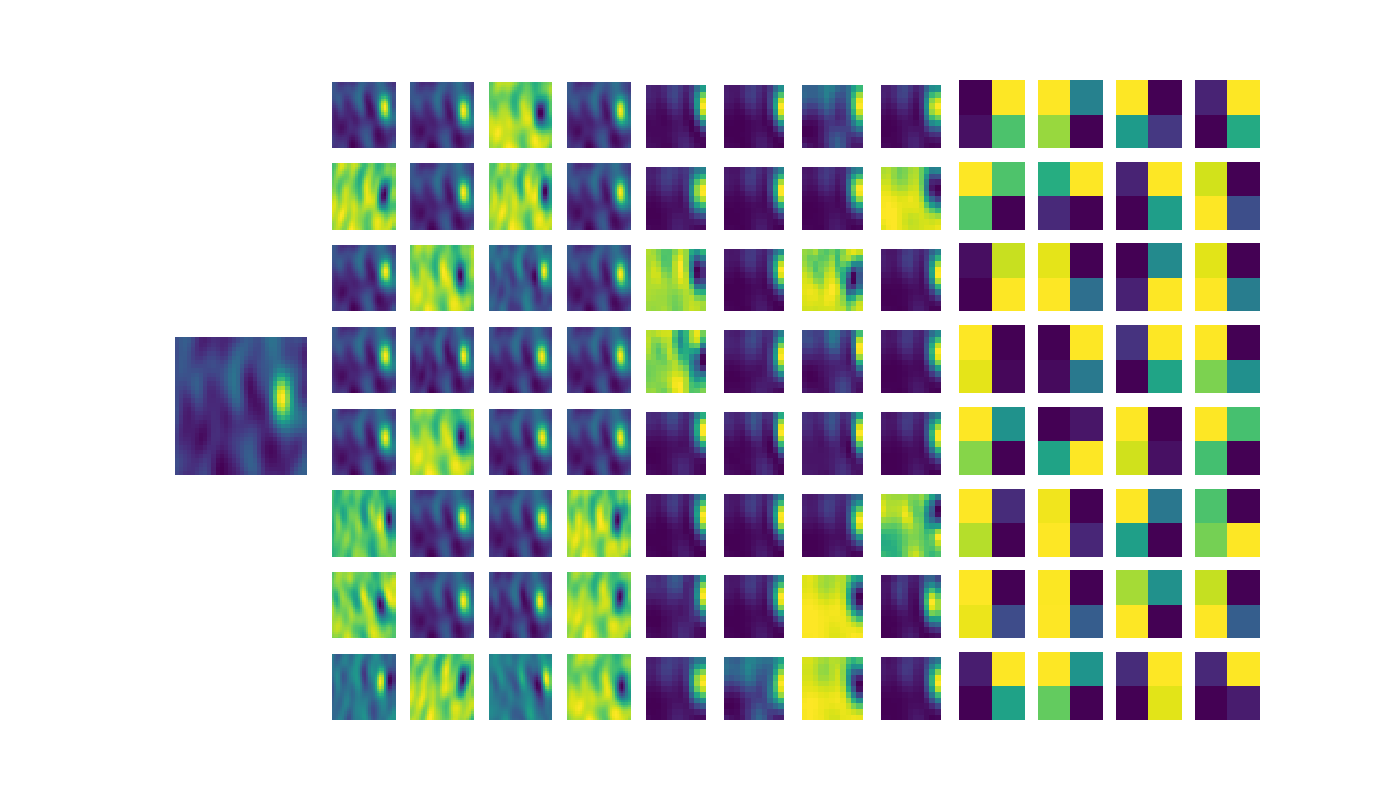
\includegraphics[width=\textwidth]{images/rgz_cnn}
        \caption{The effects of convolutional layers on an input image. The
          left-most image is the original radio image. The other images are the
          32 images output from each of the three convolutional layers.}
        \label{fig:rgz-cnn}
      \end{figure}

  \subsection{Feature Analysis}
  \label{sec:feature-analysis}

    To determine the effect of each set of features on classification
    performance, we performed a feature ablation experiment. We trained a
    logistic regression classifier on the \citeauthor{norris06} label set, each
    time using a different subset of features. The lower the resulting balanced
    accuracy, the more important the held out features. This was repeated ten
    times with different $50\%$ subsets of the training set. When holding out
    the WISE magnitude features, we also held out the CNN features, since we
    found that the CNN features tended to dominate results. These results are
    plotted in Figure \ref{fig:feature-ablation} and the means and standard
    deviations of the balanced accuracies can be found in Table
    \ref{tab:feature-ablation}.

    \begin{figure}[!ht]
      \centering
      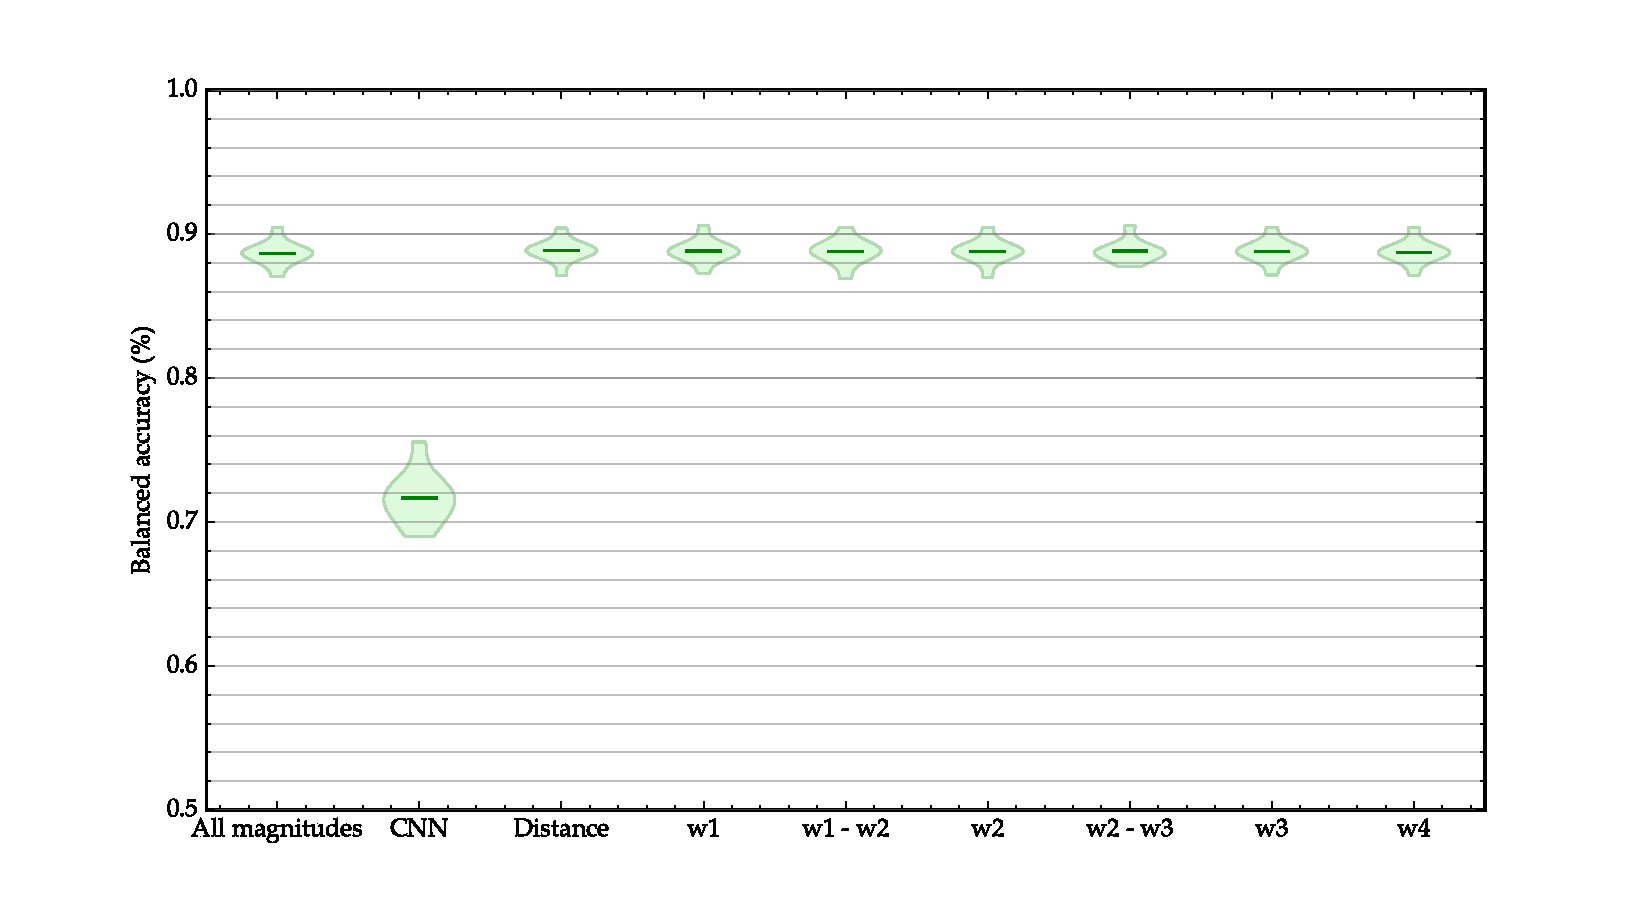
\includegraphics[width=\textwidth]{%
        images/experiments/feature_ablation.pdf}
      \caption{Balanced accuracy of logistic regression trained on the
        \citeauthor{norris06} label set with different subsets of features. The
        horizontal axis indicates which features were used for the results in
        that column.}
      \label{fig:feature-ablation}
    \end{figure}

    \begin{table}[!ht]
      \centering
      \begin{tabular}{r|c}
        \textbf{Features} & \textbf{Mean Balanced Accuracy (\%)}\\\hline
        No distance & $88.82 \pm 0.70$\\
        All features & $88.74 \pm 0.78$\\
        No magnitudes & $88.73 \pm 0.83$\\
        CNN only & $88.66 \pm 0.81$\\
        No CNN + no $w1 - w2$ & $81.32 \pm 0.81$\\
        Distance only & $79.01 \pm 0.58$\\
        No CNN & $71.67 \pm 1.71$\\
        No CNN + no $w1$ & $71.67 \pm 1.71$\\
        No CNN + no $w2$ & $71.67 \pm 1.71$\\
        No CNN + no $w3$ & $71.67 \pm 1.71$\\
        No CNN + no $w4$ & $71.67 \pm 1.70$\\
        No CNN + no $w2 - w3$ & $71.15 \pm 2.16$\\
        Magnitudes only & $56.47 \pm 0.70$\\
      \end{tabular}
      \caption{Balanced accuracy of logistic regression trained on the
        \citeauthor{norris06} label set with different subsets of features. The
        rows are sorted from highest accuracy to lowest.}
      \label{tab:feature-ablation}
    \end{table}

\section{Choosing a Binary Classifier}
\label{sec:binary-classifiers}
  
  \begin{figure}[!ht]
    \centering
    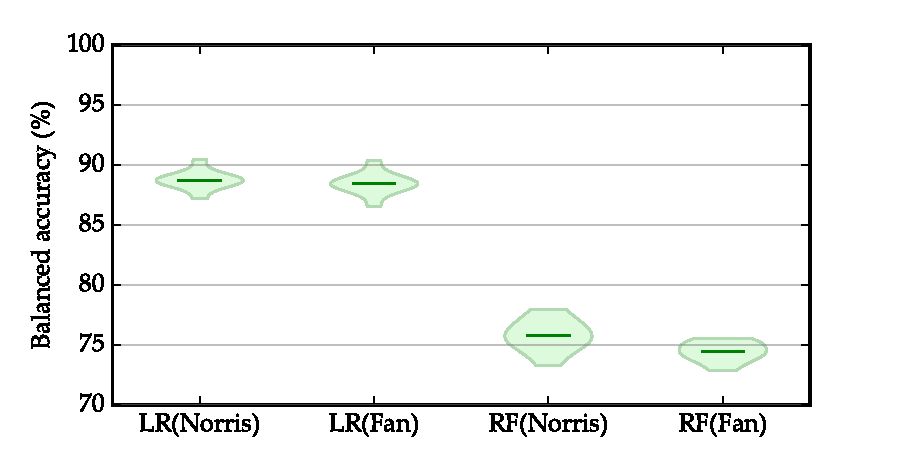
\includegraphics[width=\textwidth]{images/experiments/lr_rf}
    \caption{Comparison of logistic regression and random forests on the galaxy
      classification task, trained on the \citet{norris06} and \citet{fan15}
      label sets, and tested against the \citet{norris06} label set.}
  \end{figure}

  To compare the performance of logistic regression with random forests on the
  galaxy classification task, we performed the following experiment. We first
  generated five test sets of WISE objects. Then, using all other WISE objects
  as a training set, we trained a logistic regression classifier with $L2$
  regularisation for each test set, first using labels from \citet{norris06},
  and separately using labels from \citet{fan15}. We then computed the balanced
  accuracy for each classifier. This was repeated for random forests, with each
  tree using $\sqrt{D}$ features.

  To generate the test sets, we first selected at random half of all ATLAS
  objects. We then added all WISE objects within $1'$ of a selected ATLAS object
  to the test set. This was repeated for each test set. The motivation for first
  selecting ATLAS objects rather than drawing WISE objects directly is that WISE
  objects have overlapping features, since radio features are taken from a patch
  of sky centred on each object, and WISE objects tend to be close together.
  Objects from the test sets were then removed at random until all test sets
  were the same size.

\section{Handling Crowd Labels}
\label{sec:rgz-crowd-labels}

  \begin{figure}
    \centering
    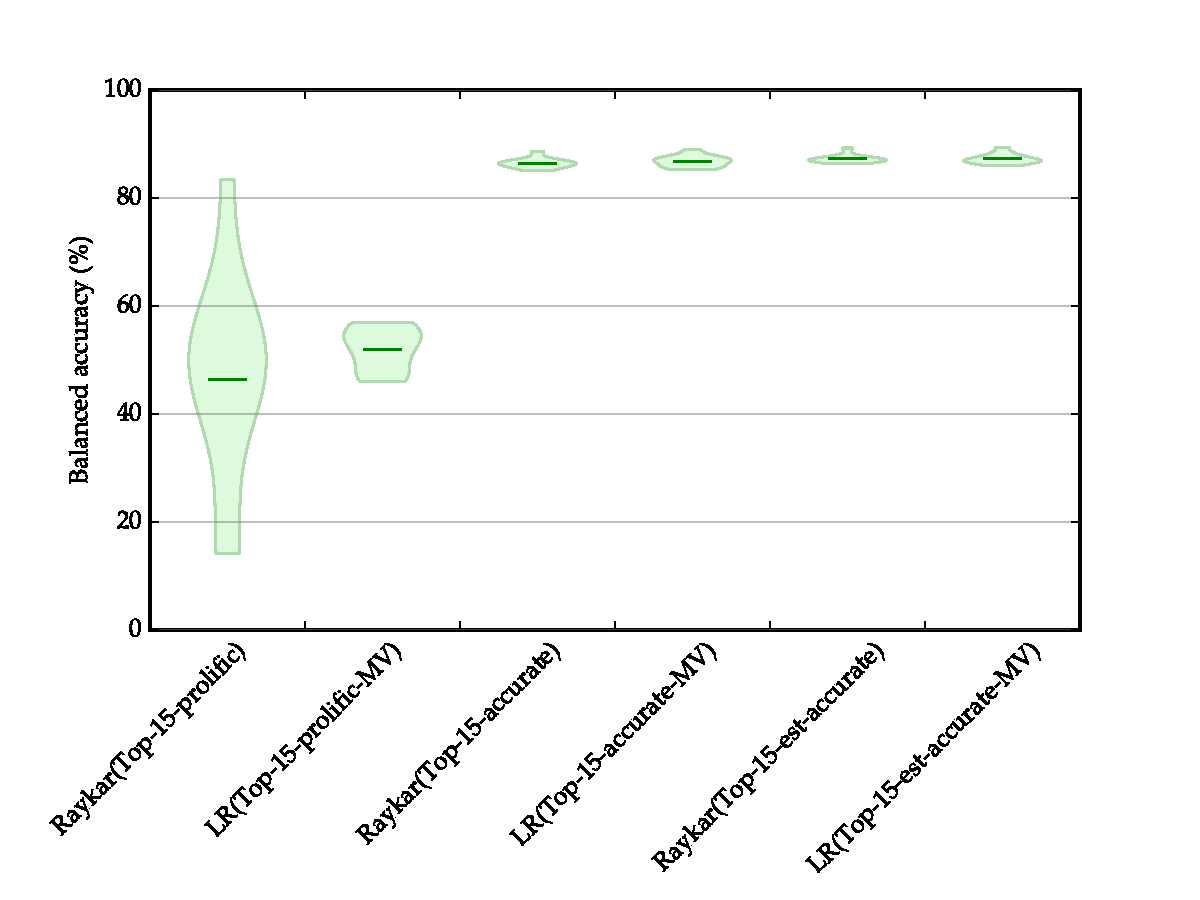
\includegraphics[width=\textwidth]{images/experiments/rgz_raykar}
    \caption{Comparison of logistic regression and \citeauthor{raykar10} on the
      galaxy classification task with different numbers of labellers.}
    \label{fig:rgz-raykar}
  \end{figure}


  While we want to train a classifier on the crowdsourced labels from the Radio
  Galaxy Zoo, it is unclear how we should aggregate the labels. Some methods for
  aggregation are described in Section \ref{sec:crowd-labels}. Which method will
  perform best on a dataset is dependent on the dataset itself, so we tested
  both variants of the \citeauthor{raykar10} algorithm and majority vote on the
  galaxy classification task.

  One key problem with the use of the \citeauthor{raykar10} algorithm is that it
  is very slow with large numbers of labellers. To mitigate this problem, we
  tested the algorithm on a subset of labellers, chosen by three different
  measures: the 10 labellers with the most labels, the 10 labellers with the
  highest balanced accuracy assessed against the \citeauthor{norris06} labels,
  and the 10 labellers with the highest balanced accuracy assessed against the
  majority vote of all labellers. While in practice on datasets such as EMU or
  FIRST there would be no equivalent to the \citeauthor{norris06} labels, we can
  treat this test as a ``best-case'' method. For each subset of labellers, the
  \citeauthor{raykar10} algorithm was tested against logistic regression trained
  on the majority vote of just these labellers. The results are shown in Figure
  \ref{fig:rgz-raykar}.

  With $T = 10$ labellers, the \citeauthor{raykar10} algorithm took $83 \pm 36$
  seconds to run. When the number of labellers was increased to $T = 15$, the
  \citeauthor{raykar10} algorithm took $152 \pm 115$ seconds to run. This helps
  to highlight how slow the algorithm becomes with increasing $T$.

\section{Galaxy Classification}
\label{sec:rgz-results}

  In this section, we present results using methods developed in this chapter.

  \subsection{Comparison of Methods}
  \label{sec:comparison-predictors}

  We trained logistic regression classifiers on three training sets:
  \begin{itemize}
    \item the \citeauthor{norris06} labels,
    \item the \citeauthor{fan15} labels, and
    \item the Radio Galaxy Zoo majority vote.
  \end{itemize}
  We also trained the \citeauthor{raykar10} algorithm with the Radio Galaxy Zoo
  labels. Each volunteer was assigned a unique index and the algorithm was run
  with $T = 2014$ total labellers.

  The classifier was then used to classify the objects in the testing set. The
  labels were compared to those found by \citet{norris06} as described in
  Section \ref{sec:norris}, resulting in $80.14\%$ balanced accuracy.
  \todo{This number is out of date.}

  \todo{ROC/precision--recall curves}

  \begin{figure}[!ht]
    \centering
    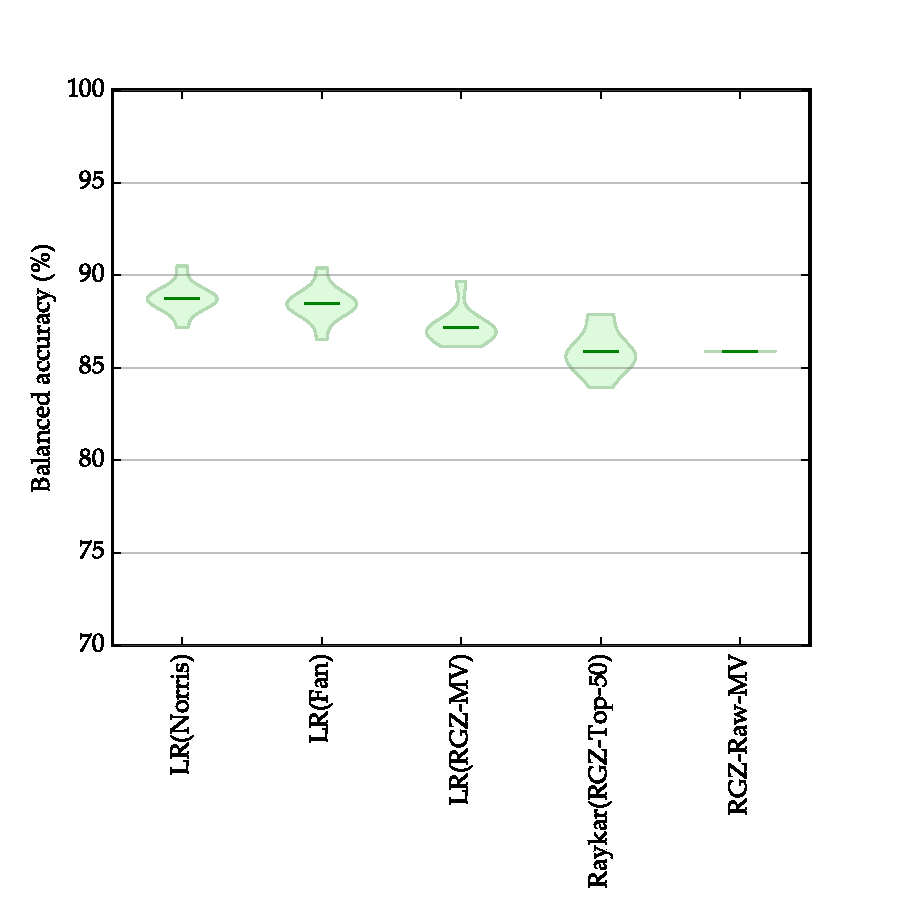
\includegraphics[width=\textwidth]{images/experiments/predictors.pdf}
    \caption{Performance of logistic regression on the galaxy classification
      task, trained on different sets of labels and tested on the galaxies
      where \citeauthor{norris06} and \citeauthor{fan15} labels agree. LR($Y$)
      indicates logistic regression trained on $Y$. RGZ-MV is the set of
      majority vote labels from the Radio Galaxy Zoo. RGZ-Raw-MV is the
      majority vote of all crowd labels and is included for comparison.}
  \end{figure}

\section{Number of Training Examples}

  \begin{figure}[!ht]
    \centering
    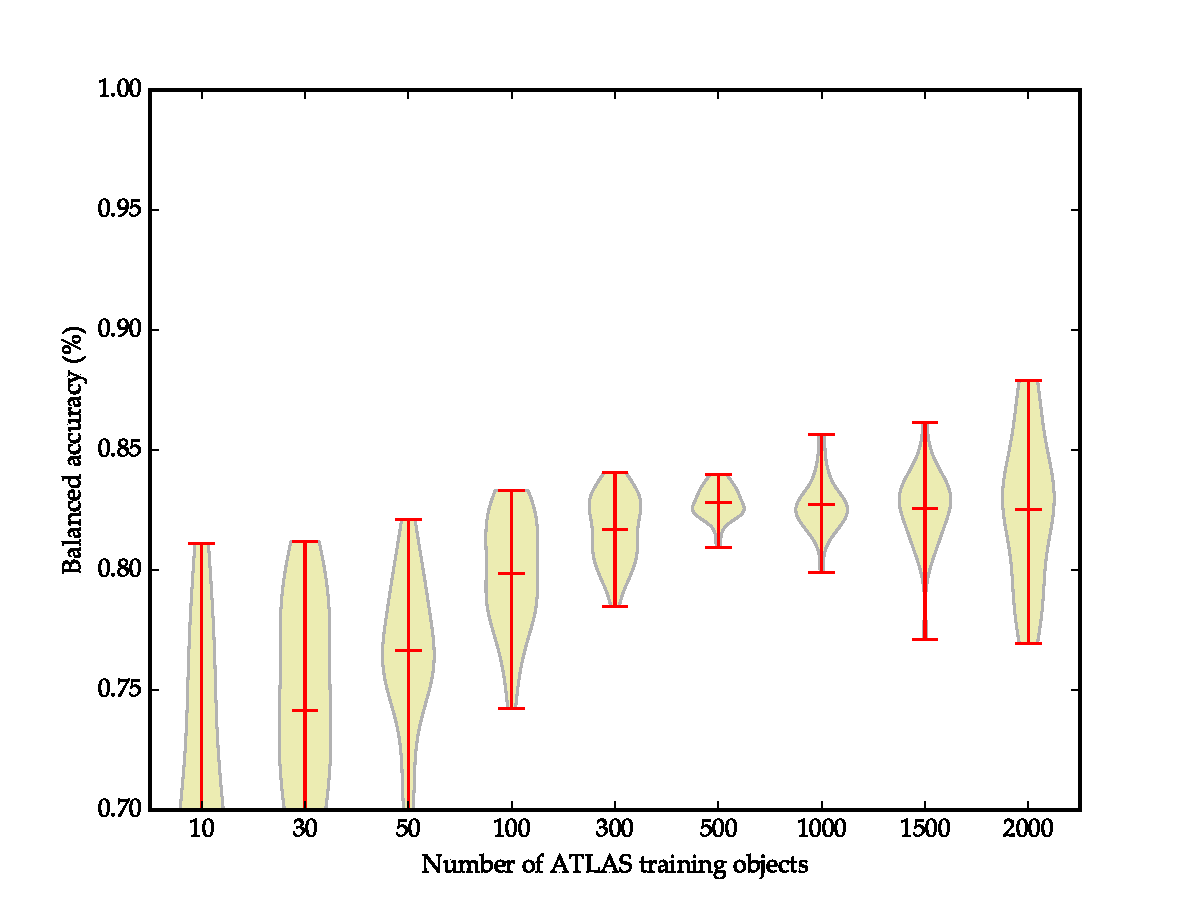
\includegraphics[width=\textwidth]{images/experiments/passive.pdf}
    \caption{Performance of logistic regression on the galaxy classification
      task, trained on different amounts of the \citeauthor{norris06} label
      set.}
  \end{figure}

  \todo{Discuss results}

%!TeX root=./thesis.tex

\chapter{Active Learning}
\label{cha:active-learning}

In this chapter we discuss active learning and look at its application to both
the galaxy classification task and to the Radio Galaxy Zoo project. In Section
\ref{sec:intro-active-learning}, we will briefly describe the key concepts of
active learning, moving to discuss querying strategies for active learning for
binary classification in \ref{sec:query-strategies}. We apply these methods in a
simple experiment in Section \ref{sec:rgz-qbc}, showing that active learning may
be useful in an astronomical context.

Section \ref{sec:active-learning-on-crowds} extends the active learning
discussion to a crowdsourcing context, and we discuss how crowdsourcing
complicates active learning. Finally, in Section \ref{sec:rgz-al-general}, we
look at the differences between the standard crowdsourcing context and citizen
science, pointing out how they differ and how this breaks assumptions of
existing methods. We end with describing an ideal experiment for active learning
applications in citizen science.

\section{Introduction}
\label{sec:intro-active-learning}
    
    In supervised learning we deal with a set of data points and their
    associated labels. This dataset may be expensive to obtain, but the main
    costs may come from collecting labels, rather than from collecting the data
    points themselves. Examples of such data include text samples
    \citep{lewis94, mccallum98}, and images \citep{loy11, lintott08}, both of
    which are now widely and cheaply available through the internet. A more
    abstract example is scientific hypotheses \citep{king04}. Labelling text and
    images is hard, error-prone, and requires humans; and performing a
    scientific experiment to test a hypothesis is considerably more expensive
    than coming up with the hypothesis. It may even be the case that we simply
    cannot label all the data because there is too much, such as in the Galaxy
    Zoo \citep{lintott08} and Radio Galaxy Zoo \citep{banfield15} projects.

    \emph{Active learning} (or \emph{query learning} \citep{settles09, seung92,angluin86})
    allows a machine learning algorithm to select specific, unlabelled examples
    to be labelled by an expert. The algorithm effectively chooses its own
    training set \citep{settles09}. The hope is that the algorithm can choose to
    label only the most useful examples \citep{mccallum98}, and the expensive
    process of labelling redundant or useless examples is avoided
    \citep{engelson99}. Intelligently selecting the training set as in active
    learning can result in massively reduced labelling costs \citep{lewis94,
    king04} or even make intractable labelling problems tractable.

    While there are many variations of active learning scenarios, we focus on
    \emph{pool-based} active learning in this thesis. In pool-based active
    learning, we already have a large pool of unlabelled data points accessible
    to our algorithms, and our algorithms can choose to present any of these
    data points to the expert. The pool-based scenario commonly arises when we
    are able to obtain a lot of unlabelled data at once, such as in astronomical
    surveys \citep{pelleg04, richards12, marshall15}.

    Active learning has already been successfully applied in astronomy.
    \citet{pelleg04} applied active learning to the Sloan Digital Sky Survey to
    find anomalies in the survey. \citet{richards12} applied active learning to
    classify variable stars from the All Sky Automated Survey. Both papers
    showed that active learning resulted in a great reduction in the number of
    labels needed to achieve their respective tasks.

\section{Query Strategies}
\label{sec:query-strategies}

    A \emph{query strategy} is the approach an active learning algorithm takes
    to selecting a new data point to label. There are many different query
    strategies, but here we focus on uncertainty sampling and
    query-by-committee.

    All pool-based query strategies take the same form. We are given some pool
    of data $\mathcal X$ and a set of labelled data $\mathcal D = \mathcal X
    \times \mathcal Y$. We want to select $\tilde x \in \mathcal X$ such that
    labelling $\tilde x$ maximises our information gain.

    \subsection{Uncertainty Sampling}
    \label{sec:uncertainty-sampling}

        \emph{Uncertainty sampling} \citep{lewis94} is perhaps the most common
        query strategy. Given a classification model $y(\vec x) = p(z \mid x)$
        with the ability to output a probability (including probabilistic
        classifiers like logistic regression, nearest-neighbour classifiers
        \citep{lewis94}, and combinations of probabilistic and non-probabilistic
        classifiers \citep{lewis94b}), the queried point $\tilde x$ is the data
        point for which the model is least certain of the classification. This
        is not well-defined and an uncertainty sampling algorithm must choose
        what ``least certain'' means. There are three common measures of
        uncertainty --- confidence-, entropy-, and margin-based --- but in the
        case of binary classification, they all reduce to one strategy
        \citep{settles09}:
        \[
            \tilde x = \underset{\vec x}{\mbox{argmax}}\ 1 - \abs{y(\vec x) - 0.5}.
        \]
        The intuition is that the further a data point is from the decision
        boundary, the more certain the classifier is of the assigned label, so
        choosing the closest data point to the decision boundary is equivalent
        to choosing the most uncertain data point. Another interpretation is that $1 - \abs{y(\vec x) - 0.5}$ is the expected probability of mislabelling $\vec x$ \citep{settles09}.

        % In the confidence-based approach, $\tilde x$ is the data point that is
        % closest to the decision boundary, i.e.

        % % In the 

    \subsection{Query-by-Committee}
    \label{sec:qbc}

        \emph{Query-by-committee} (QBC) is an ensemble-based query strategy
        first proposed by \citet{seung92}. A committee of classifiers is trained
        on the known labels, with different subsets of the labelled data to
        ensure variety in the committee. The committee then labels the
        unlabelled pool of data: Each classifier votes on each data point and
        the most commonly voted for label is assigned. The information gain
        associated with each data point is estimated by the disagreement of the
        committee on the label, and the data point with the most disagreement is
        queried.

        Disagreement can be measured in multiple ways. The most obvious is by
        simply counting the number of classifiers that disagree with the
        majority label \citep{seung92}. Other methods include computing the
        entropy of the committee vote \citep{mccallum98, dagan95}, and using
        Kullback-Leibler divergence \citep{mccallum98}.

\section{Query-by-Committee on the Galaxy Classification Task}
\label{sec:rgz-qbc}

    \begin{figure}
        \centering
        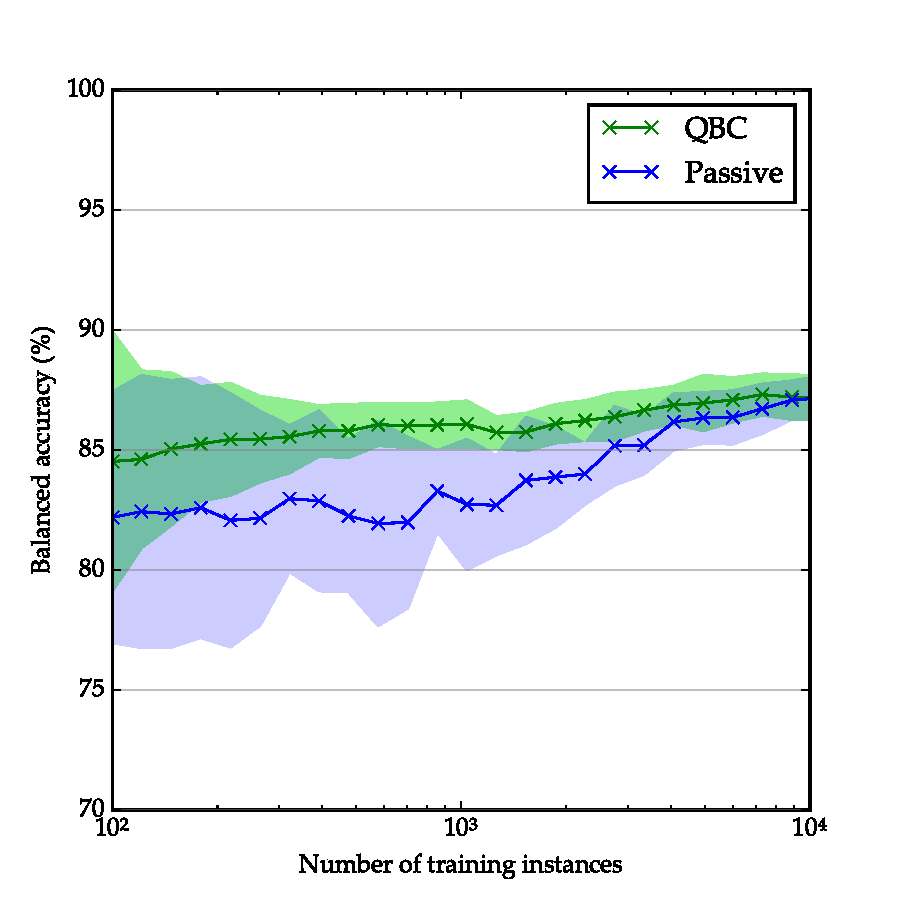
\includegraphics[width=0.8\textwidth]
            {images/experiments/rgz_qbc.pdf}
        \caption{Logistic regression trained on the \citeauthor{norris06}
            labels with different amounts of training data and two different
            query strategies.}
        \label{fig:rgz-qbc}
    \end{figure}

    We tested QBC active learning on the galaxy classification task described in
    Chapter \ref{cha:cross-identification}, comparing QBC to passive (i.e.
    random) selection as a query strategy.

    We used a committee of 20 logistic regression classifiers for the QBC test.
    Each was presented with 75\% of the known labels at random, stratified by
    the labels.

    For the passive test, we sampled 100 galaxies at random (stratified by the
    labels) and trained a logistic regression classifier on these. We then drew
    a batch of new labels, added these to the existing label set, and then
    retrained the classifier. This was repeated until the classifier had seen
    the entire training set ($10^4$ labels). The process for testing QBC was
    identical, except that instead of drawing new labels at random, the new
    labels were drawn in order of highest to lowest disagreement of the
    committee.

    After running the experiment, we observed that QBC outperformed passive
    selection. We hypothesised that this was because querying at random ignores
    the fact that there are far more negative examples than positive examples in
    the galaxy classification task. By this hypothesis, QBC would perform
    comparably to sampling from the set of positive examples and the set of
    negative examples at equal rates. To test this, we ran a third test with a
    random sampler that accounted for class imbalance. We found that this third
    test performed similarly to QBC.

    All three tested querying strategies are plotted in Figure
    \ref{fig:rgz-qbc}.

\section{Active Learning on Crowds}
\label{sec:active-learning-on-crowds}
    
    Traditional active learning assumes that we have access to one expert, who
    always issues correct labels. When labels are sourced from a crowd, these
    assumptions no longer hold: the crowd are non-experts and can give incorrect
    labels \citep{mozafari12,yan11}, and there are multiple labellers with
    different accuracies \citep{yan11}. We can now ask questions deeper than
    simply ``which label should I request?'' --- we can, for example, ask
    ``which labeller should I ask?'', or ``do I need to re-request this
    label?''.

    \citet{yan11} apply the \citet{yan10} model (Section \ref{sec:yan}) to the
    problem of active learning from crowds. We remind the reader that this model
    consists of a label model $p(z | \vec x)$ and a data-dependent labeller
    model $p(y_t | \vec x, z)$, where $\vec x$ is an instance, $y_t$ is the
    label assigned by labeller $t$, and $z$ is the groundtruth label. To extend
    this model into active learning, \citeauthor{yan11} introduce a query
    strategy where not only an instance is requested, but a specific labeller.

    First, uncertainty sampling is used with the label model to choose an ideal
    point to query. With logistic regression (Equation \ref{eq:raykar-logreg}),
    the decision boundary between positive and negative labels is a hyperplane
    $\vec w^T \vec x = 0$; uncertainty sampling would choose to query the point
    nearest (or on) this hyperplane. The labeller and instance to query are then
    chosen as solutions to the following optimisation problem:
    \begin{align*}
        \text{minimise}_{\vec x, t}\ & \eta_t(\vec x)\\
        \text{s.t. } & \vec w^T \vec x = 0.
    \end{align*}
    Intuitively, we query the instance on the decision hyperplane with the least
    noisy labeller. While this instance may not actually exist in our pool, we
    simply choose the instance closest to it (i.e. using Euclidean distance).

    This method has similar drawbacks to the \citeauthor{yan10} passive learning
    method described in Chapter \ref{cha:ml}: the number of parameters grows
    large with large numbers of annotators, and the expectation-maximisation
    algorithm only converges to a local minimum. In our implementation, training
    was also quite slow, meaning online active learning may be impractical. It
    also does not account for the possibility of relabelling instances.

    \citet{mozafari12} suggest an approach similar to uncertainty sampling, with
    uncertainty computed using a bootstrap method. A full description of this
    method is beyond the scope of this thesis. Instead, we look at the approach
    they take to handle noise. Noting that crowds may perform worse on some
    subsets of the data than other subsets, \citeauthor{mozafari12} solve an
    integer linear program to compute the redundancy required for different
    subsets of the instance pool. First, they partition the data, then estimate
    the probability of obtaining a correct crowd label for each partition. This
    estimation is accomplished by querying the crowd on a sample of instances
    from each partition. The estimated probability is then used to compute the
    redundancy required. For full details, we refer the reader to the paper
    \citep{mozafari12}.

\section{Active Learning for Radio Galaxy Zoo}
\label{sec:rgz-al-general}

\todo{Talk about citizen science and an ideal experiment}


%% Conclusion
%!tex root=thesis.tex

\chapter{Conclusion}
\label{cha:conclusion}

    Ever larger and ever more detailed radio surveys will bring new challenges
    to astronomy. In this thesis we have focused on radio cross-identification,
    a task for which existing algorithms are expected to fail and for which a
    manual approach is intractable. We have presented a new, astronomical
    model-free, supervised learning approach to this problem. We hope that this
    approach will help guide the search for innovative ways to handle the data
    produced by the Evolutionary Map of the Universe.

    In Chapter \ref{cha:cross-identification}, we framed the
    cross-identification problem first as object localisation and then as binary
    classification of galaxies. We represented galaxies with the use of a
    convolutional neural network to extract features from ATLAS radio images,
    and combined these with features from the WISE telescope. We then tested a
    variety of methods of learning for a classifier on these features, including
    logistic regression, random forests, and the \citet{raykar10} crowd learning
    algorithm. We showed that logistic regression with majority vote
    outperformed the \citeauthor{raykar10} algorithm, and that a classifier
    trained on non-expert crowd labels attains comparable accuracy to a
    classifier trained on expert labels.

    We then looked at active learning in Chapter \ref{cha:active-learning},
    applying query-by-committee to the cross-identification task. We suggested
    an experiment for using active learning on Radio Galaxy Zoo, and highlighted
    some problems with existing active learning literature when applied to
    citizen science.

    Our work here is just the start of applying machine learning to radio
    cross-identification. In Section
    \ref{sec:cross-identification-conclusion-future-work} we have suggested a
    number of avenues for future work. Performance could be improved by
    incorporating hand-selected features, using information from more
    wavelengths, and developing a better feature extraction method. Our method
    could be extended to account for infrared-faint radio objects. Machine
    learning could be applied to learn to associate related radio objects with
    each other, and then with their host galaxy. Radio Galaxy Zoo volunteers
    could be analysed to determine the best possible labeller model for use in
    crowd learning algorithms. In Section \ref{sec:al-rgz-ideal-experiment} we
    suggested an experiment for applying active learning to Radio Galaxy Zoo and
    determining an appropriate uncertainty aggregation method for the radio
    cross-identification task. Finally, in Section \ref{sec:al-citizen-science},
    we highlighted some problems with active learning and crowd learning when
    applied to citizen science, suggesting that citizen science is a unique form
    of crowdsourcing that requires additional considerations.


%%%%%%%%%%%%%%%%%%%%%%%%%%%%%%%%%%%%%%%%%%%%%%%%%%%%%%%%%%%%%%%%%%%%%%
% End text.

%!TeX root=thesis.tex

\appendix
\chapter{Crowdastro Package}
\label{cha:crowdastro}

As part of this thesis, we developed an open source Python package called
\emph{crowdastro}, containing methods for machine learning on the cross-%
identification task, and implementations of many of the methods described here.
In this appendix, we briefly describe how to obtain this package, and list the
submodules available.

\section{Obtaining Crowdastro}

    The source for crowdastro is available on GitHub at
    \url{http://github.com/chengsoonong/crowdastro}. Crowdastro can also be
    installed through pip, by running \texttt{pip3 install crowdastro}. The code
    is MIT licensed.

\section{Crowdastro}

    The crowdastro package can be imported into Python or used with the
    command-line interface.

    \todo{Finish this.}

\section{Submodules}
    \label{sec:crowdastro-submodules}

    \subsection{crowdastro.active\_learning.random\_sampler}
        \label{sec:crowdastro-random-sampler}
    \subsection{crowdastro.active\_learning.sampler}
        \label{sec:crowdastro-sampler}
    \subsection{crowdastro.active\_learning.qbc\_sampler}
        \label{sec:crowdastro-qbc-sampler}
    \subsection{crowdastro.active\_learning.uncertainty\_sampler}
        \label{sec:crowdastro-uncertainty-sampler}

    \subsection{crowdastro.crowd.raykar}
        \label{sec:crowdastro-raykar}

        \texttt{crowdastro.crowd.raykar} is an implementation of the crowd
        learning algorithm developed by \citet{raykar10}, described here in
        Section \ref{sec:raykar}. The module provides a
        \texttt{RaykarClassifier} object which implements a modified scikit-%
            learn interface.

    \subsection{crowdastro.crowd.util}
        \label{sec:crowdastro-util}

        \texttt{crowdastro.crowd.util} contains useful functions for dealing
        with crowd labels and performing related experiments shown in this
        thesis. These functions are:
        \begin{itemize}
            \item \texttt{balanced\_accuracy}, which computes the balanced
                accuracy of a classifier against a test set,
            \item \texttt{crowd\_label}, which simulates the crowd labelling
                task as described in Section \ref{sec:crowd-simulation},
            \item \texttt{majority\_vote}, which computes the majority vote of
                a set of crowd labels,
            \item \texttt{logistic\_regression}, a simple implementation of the
                logistic regression function (Equation
                \ref{eq:logistic-regression}).
        \end{itemize}

    \subsection{crowdastro.crowd.yan}
        \label{sec:crowdastro-yan}

        \texttt{crowdastro.crowd.yan} is an implementation of the crowd
        learning algorithm developed by \citet{yan10}, described here in
        Section \ref{sec:yan}. The module provides a
        \texttt{YanClassifier} object which implements a modified scikit-%
            learn interface.


\backmatter

\todo{Verify that I didn't break anything by using natbib.}

\nocite{*}
% \bibliographystyle{acmnew-xref}
\bibliographystyle{plainnat}
\bibliography{../papers}

\printindex

\end{document}
